\documentclass[review]{elsarticle}

%\usepackage{natbib}
\usepackage{lineno,hyperref}
\usepackage{amsmath}
\modulolinenumbers[5]
\usepackage{graphicx}
\usepackage{caption}
\usepackage{subcaption}
\usepackage{tikz}
\usepackage{floatrow}
% Table float box with bottom caption, box width adjusted to content
\newfloatcommand{capbtabbox}{table}[][\FBwidth]

\usepackage{blindtext}

\usepackage[colorinlistoftodos]{todonotes}   % provides \todo for margin notes

\newcommand{\BoussClaw}{\textsc{BoussClaw} }
\newcommand{\BoussClawt}{\textsc{BoussClaw}}


\newcommand{\enhet}[1]{\,\mathrm{#1}}
\newcommand{\m}{\,\mathrm{m}}
\newcommand{\mm}{\,\mathrm{mm}}
\newcommand{\kg}{\,\mathrm{kg}}
\newcommand{\s}{\,\mathrm{s}}
\newcommand{\mps}{\,\mathrm{m/s}}
\newcommand{\kmphs}{\,\mathrm{km/h}}
\newcommand{\km}{\,\mathrm{km}}
\newcommand{\Hz}{\,\mathrm{Hz}}
\newcommand{\Joule}{\,\mathrm{J}}
\newcommand{\N}{\,\mathrm{N}}
\newcommand{\Pa}{\,\mathrm{Pa}}
\newcommand{\Cgrad}{\,^\circ\mathrm{C}}
\newcommand{\minutt}{\,\mathrm{min}}
\newcommand{\hour}{\,\mathrm{h}}
\newcommand{\minut}{\ \mbox{min}}
\newcommand{\cm}{\,\mbox{cm}}
\newcommand{\cmps}{\,\mbox{cm/s}}
\newcommand{\mpss}{\,\mbox{m/s}^2}


\journal{Coastal Engineering}

%%%%%%%%%%%%%%%%%%%%%%%
%% Elsevier bibliography styles
%%%%%%%%%%%%%%%%%%%%%%%
%% To change the style, put a % in front of the second line of the current style and
%% remove the % from the second line of the style you would like to use.--00
%%%%%%%%%%%%%%%%%%%%%%%

%% Numbered
%\bibliographystyle{model1-num-names}

%% Numbered without titles--
%\bibliographystyle{model1a-num-names}

%% Harvard
%\bibliographystyle{model2-names.bst}\biboptions{authoryear}

%% Vancouver numbered
%\usepackage{numcompress}\bibliographystyle{model3-num-names}

%% Vancouver name/year
%\usepackage{numcompress}\bibliographystyle{model4-names}\biboptions{authoryear}

%% APA style
%\bibliographystyle{model5-names}\biboptions{authoryear}

%% AMA style
%\usepackage{numcompress}\bibliographystyle{model6-num-names}

%% `Elsevier LaTeX' style
\bibliographystyle{elsarticle-num-names}\biboptions{authoryear}
%%%%%%%%%%%%%%%%%%%%%%%

\begin{document}

\begin{frontmatter}

\title{A Boussinesq type extension of  the GeoClaw model - a study of wave breaking phenomena applying dispersive long wave models}

%% Group authors per affiliation:
\author[1]{Jihwan Kim}
\author[1]{Geir K. Pedersen}
\author[1,2]{Finn L{\o}vholt}
\author[3]{Randall J. LeVeque}

\address[1]{University of Oslo, Department of Mathematics, 
Oslo, Norway}
\address[2]{Norwegian Geotechnical Institute,
Oslo, Norway}
\address[3]{University of Washington, Department of Applied Mathematics, Seattle, USA}

\begin{abstract}

The nonlinear shallow water model is widely used
in the study of tsunami propagation,
but an increasing number of studies 
are dedicated to the dispersion dynamics of tsunamis.
If the wave dispersion becomes important,
Boussinesq-type models are often used. 
In this work, a general purpose Boussinesq solver, 
\BoussClawt, is introduced
for modeling non-linear dispersive tsunami propagation, 
taking into account inundation. 
The \BoussClaw model is an extension of the GeoClaw tsunami model.
It employs a hybrid of finite volume
and finite difference methods to solve
Boussinesq equations from the literature, which are 
based on the depth-averaged velocity 
and include enhanced dispersion properties.
On the other hand, in the selected formulation only some non-linearity is retained in
the dispersion term. 
In order to validate \BoussClawt, 
numerical results are compared 
to  analytic solutions, solutions obtained by pre-existing models, and laboratory experiments.
Even though the equations of   \BoussClawt\ are not fully nonlinear they perform far better
than standard Boussinesq equations with only linear dispersion terms.
Furthermore, the  wave steepening and breaking motion
is carefully scrutinized, 
and we demonstrate that the point of wave breaking
may be wrongly identified  in many of the commonly used Boussinesq models. 

\end{abstract}

\begin{keyword}
Breaking wave, Boussinesq equation, finite volume method
\end{keyword}

\end{frontmatter}

\linenumbers

\section{Introduction}

Tsunamis are  generally long waves compared to the water depth, and 
long-wave models are consequently widely used in the study of their propagation and inundation.
Through the use of numerical shock capturing techniques for modeling
the near-shore bore formation of the tsunami, {\em nonlinear shallow water} (NLSW) models
did become the standard model for modeling tsunami propagation and run-up, see e.g. 
\citep{titov1995modeling,Imamura1996b,Harig2008,BergerGeorgeLeVequeMandli11}.

The  NLSW models do not incorporate frequency dispersion, which may be included by ascending in the hierarchy of long wave expansion 
to Boussinesq type equations. 
Numerical models based on Boussinesq type equations have been used
for idealized studies of wave processes since 1966 \citep{Peregrine:1966} and 
additionally to simpler problems in coastal engineering in the following decades \citep{Brocchini:2013}. 
The accumulated effect of the frequency dispersion for the wave propagation over the open sea is 
a function of propagation time and the shape of the disturbance \citep{Glimsdal2013},
and may become important for some tsunamis, in particular for landslide sources \citep{Lovholt2015}. 
Dispersion may further be of importance, in combination with non-linear effects,
for the evolution of undular bores for tsunamis \citep{Glimsdal2013,Grue:2008,Lovholt:2008b,Behrens2015}.
In the last decades we have seen a development on long wave expansions and their numerical formulations. 
In the 1990s the modeling with  Boussinesq type equations were vitalized by 
new formulations, in particular those of  \cite{madsen1992new} and \cite{nwogu1993alternative} which  displayed improved dispersion properties in comparison to the standard formulation of \cite{peregrine1967long}.
Later still more extensions and improvements have followed as described in the reviews \cite{Madsen:2003a}, \cite{Brocchini:2013} and \cite{Kirby:2016}.

 Boussinesq-type equations differ in mathematical structure from the NLSW equations and do not
inherit characteristics in the same simple form. Hence, other strategies have been attempted for inclusion of wave breaking and  
post-breaking motion in Boussinesq models. 
\citet{schaffer1993boussinesq} employed the concept of the {\em surface roller},
first proposed by \citet{Svendsen:1984}, 
which is a volume of water passively riding at
the bore front. \citet{tissier2012new} suggested
a breaking  model based on the surface roller, the maximal front angle and the Froude number.
 Another way of incorporating breaking  was suggested by \cite{Kennedy2000} who included diffusive terms
in the momentum equation. These diffusive terms were  activated and deactivated as a steepness measure crossed thresholds. The original steepness measure was the temporal rate of surface elevation corresponding to a very steep solitary wave.
Later, \citet{lynett2006nearshore} investigated a variety of steepness measures and
then identified that the surface steepness provides 
the least sensitive breaking threshold. 
 \citet{Lovholt:2013a} similarly employed a diffusive model including transport terms, but pointed out that breaking wave Boussinesq models were prone to instabilities. 
An alternative non-linear diffusive ad-hoc breaking term was suggested by \citet{matsuyama2007study},
based on their large scale experiments of the wave propagation of undular bores on various slope angles. 
%They studied the wave breaking criteria and suggested 
%\begin{align*}
%\frac{u_s}{c} = \frac{\eta}{H} - \frac{h}{3H}
%\left(
%H\frac{\partial^2 \eta}{\partial x^2} - 2 \left(\frac{\partial \eta}{\partial x} \right)^2
%\right),
%\end{align*}
%as a wave breaking criterion.

Naturally, there is a desire to exploit the efficient and well established shock capturing framework of the NLSW models also in a dispersive context.
\cite{Antuono:2009} remolded the whole Boussinesq equations into a framework on hyperbolic form.
However, most of the recently developed Boussinesq models are based on some combination of approximate Riemann solvers, with TVD limiters, for the hydrostatic transport terms and finite differences
for dispersion terms \citep{Erduran2005,Kim2009,Shiach:2009,Roeber:2010,Dutykh:2011,shi2012high}. Among other models, this has led to the popular
\textsc{Funwave-TVD} and \textsc{Coulwave-TVD} applications. 
In most Boussinesq models that include runup on beaches, the dispersion term
is turned off in the vicinity of the shoreline to avoid interference of
the wetting-drying techniques with the
larger computational stencils from the dispersion terms. Still,
the dispersion terms are often seen to cause stability problems in
the strongly nonlinear parts of the shoaling process \citep{Lovholt:2013a}.
In fact, a practice of  
switching to the NLSW equations in the near-shore region, where large amplitude-to-depth-ratios occur, has evolved.
This allows for a relatively robust treatment of the modeling of the post breaking phase. To this end, \cite{tonelli2009hybrid} and \cite{shi2012high}, for instance, employ a wave-height to depth threshold of $0.8$  which is motivated by the maximum 
height of an undular bore, which again is related to the extreme solitary wave.
This threshold is a pragmatic choice for gentle   bottom gradients and
may be questionable under other circumstances.  

In this paper, we present a new hybrid Boussinesq type model \BoussClawt, 
of similar mold as \textsc{Funwave-TVD} and \textsc{Coulwave-TVD}, but with a different Boussinesq formulation. In particular, the dispersion term is simpler
and not fully nonlinear, as robustness is given priority over high formal order. The goal of the present article is twofold.
First, to present a careful validation of the \BoussClaw model, both towards  
laboratory experiments and reference models. Second, we use the new model
to explore the breaking phenomena in the context of Boussinesq equations.
It is investigated how different Boussinesq type models 
can represent the wave evolution until the point of breaking. In the presented example,
we are finally able to demonstrate that Boussinesq models may stably
compute the near shore tsunami propagation beyond the standard $0.8$ wave-height-to-depth threshold.
Conversely, we find that the use of this threshold  
invokes a too early formation of a breaking bore. This points indicates  
that the breaking criteria employed so far lacks generality.
%While these criteria may be attractive due to robustness, 
%they may be lacking not only for modeling the breaking phase, but %in certain situation also the pre-breaking phase.
%\marginpar{\footnotesize Move to last part of this paragraph to conclusions (or omit this)?}

This paper is organized as follows: In Section \ref{sec:model}, the base model
for the wave equations is given and the numerical scheme is outlined,
while a von Neuman stability analysis is put in \ref{append:stab}. 
Sections \ref{sec:num_tests} compares results from the \BoussClaw with analytic ones, laboratory experiments and those from other models. 
In subsection \ref{sec:num_shoaling} we scrutinize the pre-breaking shoaling of Boussinesq type equations through comparison with full potential theory, while the post-breaking evolution is investigated in  subsection  \ref{sec:discuss_breaking}.

\section{Model Description}
\label{sec:model}

Boussinesq-type equations are   derived 
on the assumption that the ratio of depth to wavelength, $\mu$,
is small. In addition one may assume that 
the ratio of wave amplitude to depth, $\epsilon$, is small.
Different kinds of long wave assumptions are then generally characterized
by relative errors in terms of these two parameters.
Herein we will neither derive Boussinesq equation nor make the equations 
dimensionless as such. Still, $\mu$ and $\epsilon$ will sometimes be used to indicate relative errors.
Moreover, when presenting results we will often use dimensionless quantities which are marked by a star.
The horizontal and vertical and temporal coordinates are denoted by $x$, $y$ and $t$, respectively, 
while the depth averaged horizontal velocity and the surface elevation are denoted by $u$ and $\eta$, respectively.
Dimensionless variables are then defined as
\begin{equation}
\label{eq:norm_coord}
t^*=\sqrt{\frac{g}{h_0}}t,\quad x^*=\frac{x}{h_0},\quad \eta^*=\frac{\eta}{h_0},\quad u^*=\frac{u}{\sqrt{gh_0}},\quad\mathrm{etc.}
\end{equation}
where $h_0$ is a reference depth which is chosen as the maximum equilibrium depth. Dimensional variables will be used in the sections \ref{sec:model},
\ref{sec:comp_test}, \ref{append:stab}, \ref{append:energy}, and finally the figures \ref{fig:bp5_water_tank}, \ref{fig:bp5b_gauges} and \ref{fig:init_setup}. Elsewhere, dimensionless variables are employed. Sometimes the dimensionless 
quantities are spelled out, such as $x/h_0$, but mostly starred quantities are used.  

%\ref{sec:sol_prop}, \ref{sec:shoaling_runup}, \ref{sec:shoaling_breaking}, \ref{append:stab}
%figures \ref{fig:soliton_ts} \ref{fig:soliton_error_energy}

\subsection{\BoussClaw - a new long wave model for tsunami propagation and run-up}
In this work, a new numerical model, 
called \BoussClawt, is introduced. 
It is an extension of \textsc{GeoClaw} \citep{clawpack},
and solves 
the Boussinesq-type equations derived by \citet{schaffer1995further}.
The extended model is formulated in two horizontal directions, 
but herein we focus on the description of plane waves for simplicity. 
Tests and details on the 
performance with two horizontal directions are found in \cite{kim2014finite}.

The \BoussClaw model
employ a  finite volume technique for the NLSW part of the equations and a finite 
difference discretization in 
fractional steps.
The \textsc{GeoClaw} software is 
a part of \textsc{Clawpack} \citep{clawpack}
developed mainly by
\citet{leveque1997wave}, \citet{george2008augmented}
and \citet{BergerGeorgeLeVequeMandli11},
which is designed to solve the nonlinear shallow water equations.


%with properties such as high-resolution, total variation diminishing (TVD) and adaptive mesh refinements (AMR).
% The wave propagation algorithms by LeVeque (1997) \cite{leveque1997wave} is implemented, and the steady state is preserved. 

\subsubsection{Boussinesq-type equations}

\citet{schaffer1995further} derived 
Boussinesq-type equations
where addition of a higher order  $O(\mu^4)$  term enabled optimization of
linear dispersion properties.
We restrict ourselves to the choice $B_2=0$ 
from the formulation of \citet{schaffer1995further}.
The equations then read 
\begin{flalign}
& H_t + (Hu)_x  = 0, \label{eq:madsen_cons_mass} & \\ 
& (1-D)\big\lbrack(Hu)_t\big\rbrack + \left( Hu^2 + \frac{g}{2}H^2 \right)_x - gHh_x -Bgh^2\left(h\eta_x\right)_{xx} =-f_D, \label{eq:madsen_momx} &
\end{flalign}
where we have added a Manning type friction term, denoted by $f_D$ and defined in eq.~(\ref{eq:Manning})
The operator $D$ is defined in terms of the dummy variable $w$ according to
\begin{flalign}
 D (w) &= \left(B+\frac{1}{2} \right)h^2 w_{xx} -\frac{1}{6} h^3 \left(\frac{w}{h}\right)_{xx}, & \label{eq:madsen_new_op}
\end{flalign}
for any $w(x,t)$.
In the above equations $H(x,t)$ and $u(x,t)$ are the total flow depth and the depth averaged velocity of the water, respectively, 
$h(x)$ is the still water depth, $\eta(x,t)$ is the surface elevation,
and thus $H(x,t)=h(x)+\eta(x,t)$. 
Moreover, $g$ is the acceleration of gravity, 
and $B$ is a dispersion parameter. 
\citet{madsen1992new} 
have chosen  $B=1/15$ for which the dispersion relation from the Boussinesq equations
follows linear potential theory to a higher order in wave number times depth.   
When $B=0$, this set of the Boussinesq-type equations
approximately reduces to that of \citet{peregrine1967long}
as the linear dispersion relations are identical. 
However, unlike Peregrine's momentum equation 
the hydrostatic parts of (\ref{eq:madsen_momx}) 
are written in a conservative form. Moreover, some nonlinearity is introduced
in the dispersion term. 
%\todo{Why do S and M introduce them ?} 
Even though (\ref{eq:madsen_cons_mass}), 
(\ref{eq:madsen_momx}) and (\ref{eq:madsen_new_op}) do not constitute a fully nonlinear set of Boussinesq equations, inheriting relative errors of order $\mu^2,\,\epsilon\mu^2$, 
they do describe shoaling of solitary waves markedly
better than, for instance, the Peregrine equations, as will be demonstrated in 
section  \ref{sec:num_shoaling}.


The \BoussClaw model
solves the Boussinesq-type equations (\ref{eq:madsen_cons_mass}) and (\ref{eq:madsen_momx}) numerically
with a hybrid combination of the finite volume and finite difference methods that will be explained in a moment. 
There have been several studies of this type of hybrid schemes.
For example, see \citet{tissier2011serre}, \citet{shi2012high} and \citet{dutykh2013finite}.


To facilitate a fractional step method, as outlined below, we move the hydrostatic terms of (\ref{eq:madsen_momx}) inside the $(1-D)$ 
operator, while balancing with extra terms in the $\Psi$, to obtain
\begin{flalign}
& (1-D)\big\lbrack (Hu)_t + \left(Hu^2 + \frac{g}{2}H^2 \right)_x - gHh_x\big\rbrack = -\Psi(x,t)-f_D, & \label{eq:hybrid_src}
\end{flalign}
where
\begin{flalign}
\Psi(x,t)= & \left(B+\frac{1}{2} \right) h^2 \left( (Hu^2)_{x} + g H \eta_x \right)_{xx} \nonumber\\
& -\frac{1}{6}h^3 \left( \frac{ (Hu^2)_x +gH\eta_x }{h} \right)_{xx}
-Bgh^2\left(h\eta_x\right)_{xx}. &
\label{eq:madsen_new_disp_x}
\end{flalign}


\subsubsection{Numerical scheme}
\label{sec:Num_scheme}
The equations (\ref{eq:madsen_cons_mass}) and (\ref{eq:hybrid_src}) are 
written in a conservative form with respect to the leading order terms in $\mu$, 
but with the $\Psi$
term as a pseudo source.
Such equations may be solved  
by a {\em fractional step method} as described in  
\citet{leveque2002finite}.
First, it is observed that (\ref{eq:hybrid_src}) may be formally
rewritten as 
\begin{flalign}
& (Hu)_t =- \left\lbrace\left(Hu^2 + \frac{g}{2}H^2 \right)_x - gHh_x\right\rbrace -(1-D)^{-1}\Psi(x,t)-(1-D)^{-1}f_D, & \label{eq:hybrid_inv}
\end{flalign}
At the first stage of the hybrid scheme, we integrate $Hu$ over a time step
taking into account all hydrostatic terms, namely 
those within the braces on the right hand side, and omitting the source terms involving $\Psi$. 
When this is combined with the continuity equation
(\ref{eq:madsen_cons_mass}) this simply corresponds to advancing 
the shallow water equations one time step forward. 
To this end we employ \textsc{Geoclaw},
a high-order accurate finite volume solver 
for the shallow water equations.

Next, the Manning resistance term is accounted for. To this end we
ignore the coupling of bottom friction and dispersion (replace $(1-D)^{-1}$ by
$1$ in (\ref{eq:hybrid_inv}))  and employ the semi-implicit solver in 
\textsc{Geoclaw} for $(Hu)_t=-f_D$. 


In the final stage, we retain the $H$ value, but integrate $Hu$ (essentially being the momentum density) further 
from the two first stages by solving
\begin{flalign}
& \left(1-D \right)\big\lbrack (Hu)_t\big\rbrack = -\Psi . & \label{eq:hybrid_mom_fdm}
\end{flalign}
Since the differential operator $D$ contains spatial derivatives,
a systems of difference equations must then be solved. 

The spatial and time discretization should be carefully chosen 
for the stability of the second stage. 
In our numerical scheme, the second order centered scheme
is used for the spatial discretization, 
and a four stage Runge-Kutta method is used for the time integration.
The von Neumann stability analysis of this numerical scheme 
is outlined in \ref{append:stab}.

Suppose the spatial domain is divided into $n$ grid cells with 
the spatial grid size $\Delta x$.
Arrays of nodal values for flow depth and $Hu$, respectively, are
defined as
\begin{flalign*}
\textbf{H} & =
(H_1,H_2, \dots , H_n)^T, & \\
\textbf{M} & =
(H_1u_1,H_2u_2, \dots , H_nu_n)^T. &
\end{flalign*}

With time increment $\Delta t$ the fourth order Runge-Kutta scheme
can be written as follows,
\begin{flalign}
\textbf{M}^1 = \textbf{M}, \quad 
\textbf{M}^2 = \textbf{M} + \frac{\Delta t}{2}\textbf{S}^1, \quad
\textbf{M}^3 = \textbf{M} + \frac{\Delta t}{2}\textbf{S}^2, \quad
\textbf{M}^4 = \textbf{M} + \Delta t \textbf{S}^3,
\label{eq:rk4_S}
\end{flalign}
where $\textbf{M}^k$ are intermediate value arrays
%\marginpar{How are values for $H$ obtained in the steps; linear interpolation ?} 
and $\textbf{S}^k$ are
correspondingly arrays for the time derivatives of $Hu$, obtained by
solving 
\begin{flalign}
(I-\bar{D})\textbf{S}^k & 
= -\bar{\Psi}(\textbf{H},\textbf{M}^k), \quad \textrm{for~} k=1,\dots,4. &
\label{eq:rk4_1}
\end{flalign}
Here $\bar{\Psi}$ and $\bar{D}$ represent centered spatial discretization for the term $\Psi$ and the operator $D$, respectively. These
are given explicitly below.
Finally the value of $\textbf{M}$ at the new time level is
obtained by
\begin{flalign}
\textbf{M}^+ & = \textbf{M} + \frac{\Delta t}{6} \left[
\textbf{S}^1+2\textbf{S}^2+2\textbf{S}^3+\textbf{S}^4
\right]. 
\label{eq:rk4_assemble}
\end{flalign}
In (\ref{eq:rk4_1}), 
$\bar{D}$ is a tri-diagonal $n\times n$ matrix with elements 
\begin{flalign*}
 \bar{D}_{i,i-1} = & \frac{1}{\Delta x^2} \left[
 \left(B + \frac{1}{2} \right) h_i^2 
-\frac{1}{6} \frac{h_i^3}{h_{i-1}} \right],  & \\
 \bar{D}_{i,i} = & \frac{1}{\Delta x^2}
 \left(-2B - \frac{2}{3} \right) h_i^2 ,  & \\
 \bar{D}_{i,i+1} = & \frac{1}{\Delta x^2} \left[
 \left(B + \frac{1}{2} \right) h_i^2 
-\frac{1}{6} \frac{h_i^3}{h_{i+1}} \right].  & 
\end{flalign*}
Correspondingly, the $i$-th element of $\bar{\Psi(\textbf{H},\textbf{q})}$ is 
\begin{flalign*}
\bar{\Psi}_i 
&=  \left(B+\frac{1}{2} \right) \frac{h_i^2}{2\Delta x^3} 
\Bigg[
\left(\frac{M_{i+2}^2}{H_{i+2}} -2\frac{M_{i+1}^2}{H_{i+1}} 
+2\frac{M_{i-1}^2}{H_{i-1}}-\frac{M_{i-2}^2}{H_{i-2}} \right) \\
& +g\left(H_{i+1}\left(\eta_{i+2}-\eta_{i}\right)
-2H_{i}\left(\eta_{i+1}-\eta_{i-1}\right) 
+H_{i-1}\left(\eta_{i}-\eta_{i-2}\right) \right)\Bigg]  \\
& -\frac{1}{6}\frac{h_i^3}{2\Delta x^3} \Bigg[
 \frac{M_{i+2}^2/H_{i+2}-M_i^2/H_i}{H_{i+1}}
 -2\frac{M_{i+1}^2/H_{i+1}-M_{i-1}^2/H_{i-1}}{h_{i}} \\
& +\frac{M_{i}^2/H_{i}-M_{i-2}^2/H_{i-2}}{H_{i-1}}
 \\
 &+ g \left( \frac{H_{i+1}(\eta_{i+2}-\eta_{i})}{H_{i+1}} 
 -2 \frac{H_{i}(\eta_{i+1}-\eta_{i-1})}{h_{i}} 
 + \frac{H_{i-1}(\eta_{i}-\eta_{i-2})}{H_{i-1}} 
 \right) \Bigg] \\
& -\frac{Bgh_i^2}{2\Delta x^3}
\left( H_{i+1}\left(\eta_{i+2}-\eta_{i} \right)
-2H_{i}\left(\eta_{i+1}-\eta_{i-1} \right)
+H_{i-1}\left(\eta_{i}-\eta_{i-2} \right) \right), &
\end{flalign*}
for $i=1,2,\dots,n$.
\subsubsection{Additional numerical features}
\label{sec_add_num}
Following \cite{tonelli2009hybrid} and \cite{shi2012high} we may represent wave breaking in a heuristic fashion 
through  invocation of a threshold $\epsilon_B:=\eta/h=0.8$ in \BoussClaw.
When the threshold is reached, the wave breaking is supposed to be initiated, 
and the dispersive terms are suppressed throughout the computational domain. 
This is adequate for the applications presented herein, which involve a single solitary wave. For other applications the switch to the NLSW equations 
should be made for only a subregion of the computational domain.

Bottom friction is important for inundation on gentle slopes. 
Figure \ref{fig:BoussClaw_runup} 
exemplifies that the friction reduces the run-up height.
\BoussClaw uses the Manning-type friction as follows,
\begin{equation}
\label{eq:Manning}
f_D = -\frac{g C_d^2 u |u|}{H^{5/3}}.
\end{equation}
In Section \ref{sec:num_tests}, a non-dimensional Manning friction
coefficient is used as $C_d^* = C_d \sqrt{\frac{g}{h_0}} h_0^{-1/3}$,
with the typical range between 0.01 and 0.04 \citep{te1959open}.


In the wetting-drying process during runup a parameter 
for the dry tolerance $d_{tol}$ is chosen
such that $H$ is put to $0$ if $H<d_{tol}h_0$, where $h_0$ is the reference depth (maximum equilibrium depth).
In this work, the parameter $d_{tol}$ is set to $10^{-4}$. 
%As noted by \cite{antuono2012role}, the shoreline dynamics can change  depending on the bottom friction coefficient and the water depth tolerance. 
The dispersion terms of the Boussinesq equations imply an extended computational
stencil as compared to that for the NLSW equations. To prevent this stencil 
from including dry nodes and thereby produce irregularities and even instabilities, the dispersion terms are switched off when $h<Nd_{tol}h_0$ (close to the equilibrium shoreline), where the number $N$ is set to 100 for the simulations herein.
Accordingly, for the dry land inundation, the \BoussClaw invariably
utilizes the NLSW solver of the \textsc{Geoclaw} software,
which can handle 
wet and dry states with the depth positivity property.
Details can be found in \cite{george2008augmented}.
The near-shore truncation of the dispersive terms produce small wriggles (see figure \ref{fig:bim_serre_boussclaw_slope10}, right panel) that remain small as $\Delta x$ is 
reduced and do not influence the overall solution. 


\subsection{Models for comparison}
The performance of the Boussinesq model presented here is partly
assessed by comparison with numerical results from a full potential
flow model which is described in \citet{Lovholt:2013a} and references therein. The model is based on a boundary 
integral technique and is run  with fully nonlinear solitary
wave solutions as initial conditions. During shoaling and breaking this
model can describe the evolution of a plunger, but breaks down
when the plunger reaches the free surface. Hence, the potential flow 
results are used to determine the point of breaking due to shoaling 
and to
evaluate the evolution of  amplitude and wave 
shape of the current model until this point.   
Below we refer to the full potential model as the BIM (Boundary
 Integral Method) model.

Comparison with a pre-existing, fully nonlinear Boussinesq model is
facilitated by the application of a Lagrangian model, described
in \citet{Lovholt:2013a}. Apart from the use of
Lagrangian coordinates the equations employed in this model are
 similar to (\ref{eq:madsen_cons_mass}) and (\ref{eq:madsen_momx}).
They differ only in the nonlinearities in the
dispersion terms and in that  the dispersion optimization terms are added in a fully nonlinear fashion.
Presently, the Lagrangian model has no established bore capturing 
facility and is hence valid only to the point of breaking.
Results from this model will be referred to as {\em Serre}, even though
the dispersion enhancement is invoked. 
 
Results for the Peregrine-type equations are obtained by the
GloBouss model. This is a model for oceanic tsunami propagation which
is based on  discretization on a staggered grid. Further details are found in 
\citet{Lovholt:2008b}.

For comparison also the version 2.1 of the  \textsc{Funwave-TVD} model
by \citet{shi2012high} is used. The
\textsc{Funwave-TVD} model shares important features with \BoussClawt, employing a hybrid 
of the finite volume and finite difference
scheme to solve the fully non-linear higher order dispersive Boussinesq model numerically.
While we refer to \citet{shi2012high} for details, we briefly note that \textsc{Funwave-TVD} is based on the fully nonlinear 
Boussinesq equations of \citet{Chen06}. The numerical spatial representation in \textsc{Funwave-TVD} is MUSCL TVD scheme 
to discretize for the flux and first order terms, 
whereas a central finite difference
scheme \citep{Wei95} is utilized for the higher order momentum terms. A Runge-Kutta scheme is employed for the time stepping.

\section{Comparing \BoussClaw simulations with well-defined tests}
\label{sec:num_tests}
Four different test of \BoussClaw is presented.  
In Section \ref{sec:sol_prop} solitary wave propagation is considered.
Even if this test is simple it includes dispersion and nonlinearity. 
Moreover, a scrutiny of the variation of energy with time and resolution  shows that the artificial dissipation induced by the TVD part of the numerical scheme
 is very small for smooth waves.
Solitary wave propagation in a moderately complex bathymetry is
computed in  section \ref{sec:comp_test} and compared with experiments.
Finally, more detailed studies of shoaling and runup properties
of the model concern non-breaking (section \ref{sec:10degrunup}) and 
breaking (section \ref{sec:wave_break}) runup. Together these
tests should provide a solid assessment of  \BoussClawt. The results in  the sections 
  \ref{sec:sol_prop}    and \ref{sec:shoaling_runup} are mainly presented  in 
normalized coordinates, $t^*$ and $x^*$, as defined by (\ref{eq:norm_coord}),
whereas results in section \ref{sec:comp_test} are more conveniently expressed with 
dimensions retained.


\subsection{Solitary wave propagation}
\label{sec:sol_prop}
%\todo{Geir will fix the scaling in this subsection}

For validation of the numerical approach 
solitary wave propagation is computed in constant water depth.
For the initial conditions, 
the analytic solitary wave solution 
of the Serre's equations is used
since exact analytic solutions are unknown 
for
the set (\ref{eq:madsen_cons_mass}) and 
(\ref{eq:madsen_momx}).
In dimensionless coordinates the solitary wave solution of Serre's equations is given as
\begin{flalign}
\label{eq:anal_serre}
 \eta^*(x^*,t^*) = \alpha\, \textrm{sech}^2 \left( \kappa (x^*+ct^*-x^*_i)\right),\quad
\textrm{and}\quad u^* = -c \frac{\eta^*}{1+\eta^*},
\end{flalign}
where $x^*_i$ is the initial location of the crest peak, and 
\begin{flalign}
\begin{split}
& \kappa = \sqrt{\frac{3\alpha}{4(\alpha+1)}}, \quad \textrm{and}
 \quad c = \sqrt{1+\alpha}.
\end{split} &
\end{flalign}
In these expressions $h_0$ is the equilibrium  depth and $\alpha$ is the dimensionless amplitude. For the Serre model with enhanced dispersion we employ a modified version of
(\ref{eq:anal_serre}) while the BIM model is initiated with Tanaka's solution.
Details are given in \citet{Lovholt:2013a}.

In Figure \ref{fig:soliton_ts} 
surfaces from a \BoussClaw simulation with $\Delta x^*=\Delta x/h_0 = 0.05$ are shown for  
amplitude  $\alpha=0.2$.
The computational results are in good agreement 
with the analytic solutions concerning height, shape and propagation speed. 
The amplitude decreases very gently as the wave propagates.
%\todo{Change labels on axes to $\eta/h$ and $x/h$ and change $t$ to $t^*$ in figure 1.} 

%The discrepancy may be  partially due to the numerical errors
%and partly to the fact that 
%the analytic solution for Serre's equations satisfies
%the present Boussinesq-type equations only approximately.

\begin{figure}[!htb]
\centering
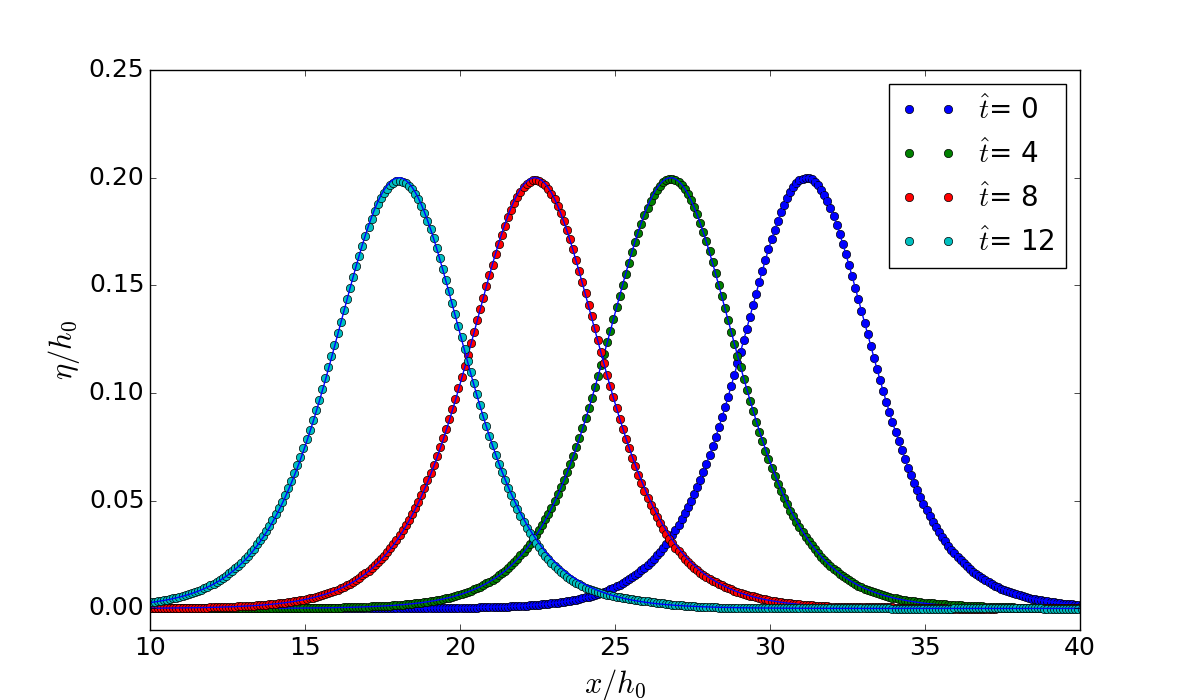
\includegraphics[width=.8\textwidth]{_fig/soliton_ts.png}
\caption{Analytic and computed solitary wave surfaces for 
$\alpha=0.2$ and $\Delta x^*=0.1$. 
The curves are marked by the normalized time
$t^*$. 
The wave propagates from right to left,
and the analytic solutions are solid lines.}
\label{fig:soliton_ts}
\end{figure}

\begin{figure}[!htb]
    \centering
    \begin{subfigure}[b]{0.45\textwidth}
        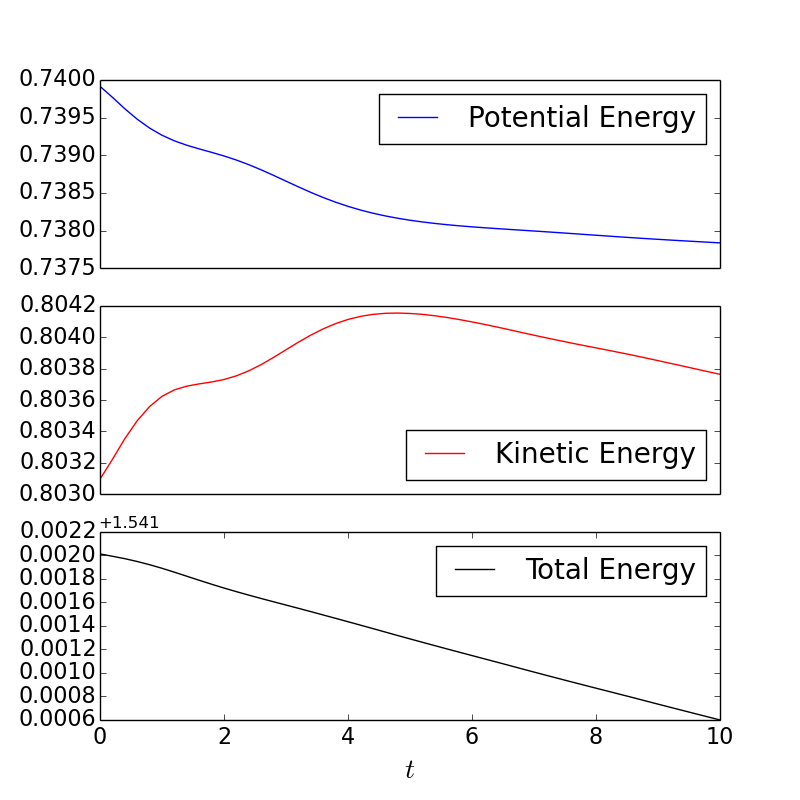
\includegraphics[width=\textwidth]{_fig/soliton_energy.png}
        \caption{}
        \label{fig:soliton_energy}
    \end{subfigure}
    \begin{subfigure}[b]{0.45\textwidth}
        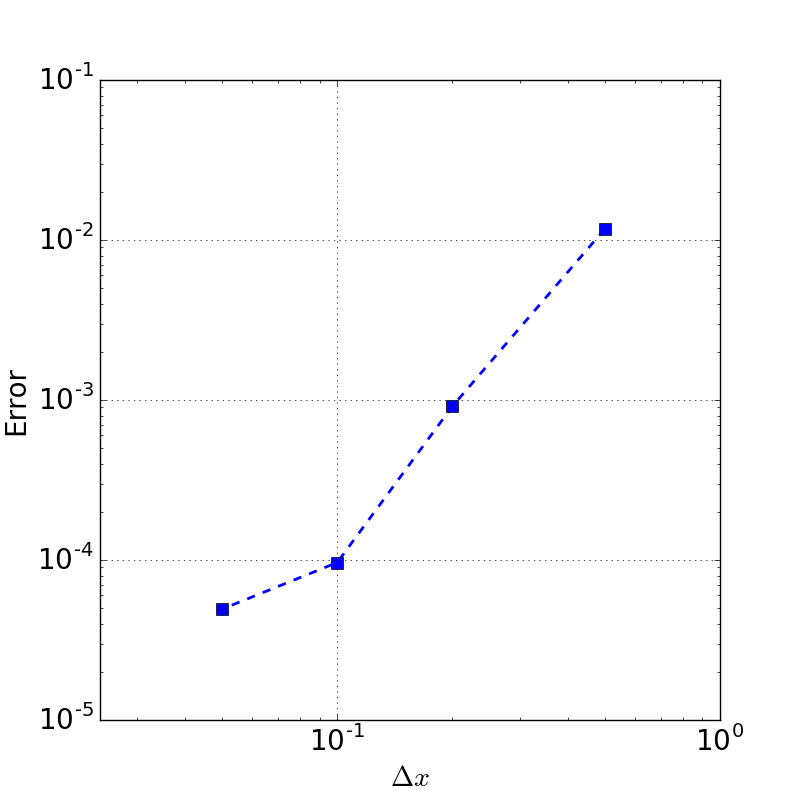
\includegraphics[width=\textwidth]{_fig/soliton_energy_dx.png}
        \caption{}
        \label{fig:soliton_energy_dx}
    \end{subfigure}
    \caption{Evolution of energies for a solitary wave with $\alpha=0.2$.
    (a): Different parts of the dimensionless energy $E^*=E/E_c$.
    for $\Delta x^* = 0.1$. (b): 
    log-log plot of relative error of energy
    at $t^*=10$ for $\Delta x^* = 0.05, 0.1, 0.2$ and $0.5$.}
    \label{fig:soliton_error_energy}
\end{figure}

The  integrated wave energies (per width) for the NLSW 
and Boussinesq equations are $E_0$ and $E_0+E_1$, respectively, as
described in \ref{append:energy}. These quantities are made dimensionless by $E_c=\rho g h_0^3$, which is minus two times the equilibrium potential energy per width.
In Figure \ref{fig:soliton_energy} the time evolution of these energies are
 shown for $\alpha=0.2$ and $\Delta x^* = 0.2$.
There are tiny fluctuations both in the potential and kinetic energy that is evident when we zoom in,
and the total energy decrease 
shows that the numerical procedure has a slight dissipation.
In Figure \ref{fig:soliton_energy_dx},
the relative error of the energy at $t^*=10$, 
\begin{flalign*}
Error = \frac{\left| E^*_{t^*=0}-E^*_{t^*=10} \right|}{\left|E^*_{t^*=0}\right|}, &
\end{flalign*}
is shown for different $\Delta x^*$.
For a solitary wave on a constant depth,
the energy dissipation decreases with the grid increments.

\subsection{Waves on a composite slope}
\label{sec:comp_test}
A physical model was constructed at the Coastal Hydraulic Laboratory of the U.S. Army Corps of Engineers
in order to address beach erosion and severe flooding problems \citep{chl_bp5}. 
The model beach consisted of three piece-wise linear slopes of 1:53, 1:150, and 1:13 with a vertical wall at the shoreline as shown in Figure \ref{fig:bp5_water_tank}.
In the laboratory, the wave maker was located at $23.23\m$ from vertical wall and produced incident waves that were close to solitary waves.
The gauge data from three cases are provided 
where the relative amplitude $\alpha$ equals  $0.038$, $0.259$ and $0.681$, respectively,
where $h_0=21.8\cm$ is  the depth at the wave maker.

\begin{figure}[!htb]
\centering
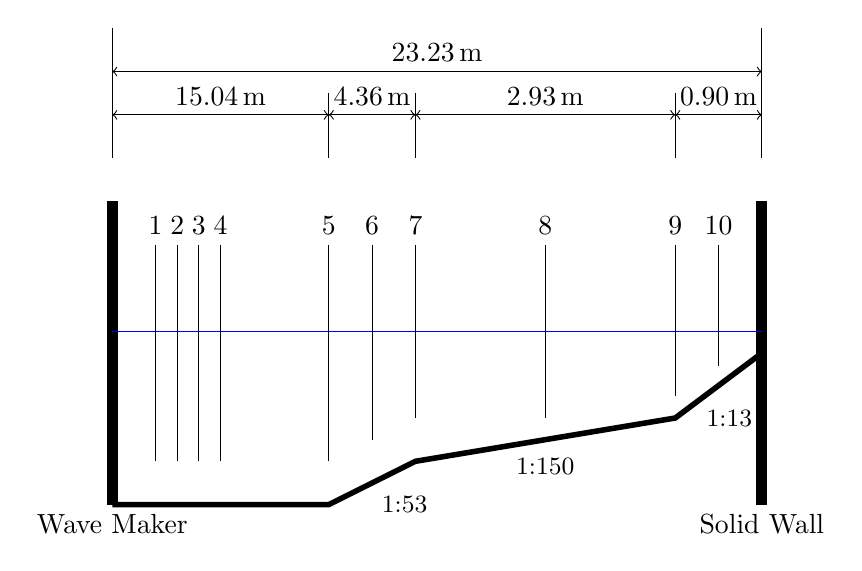
\begin{tikzpicture}[scale=.55]
 \draw[line width=4pt] (0,-4) -- (0,3);
 \draw[line width=2pt] (0,-4) -- (5,-4) -- (7,-3) --(13,-2) -- (15,-0.5);
 \draw[line width=4pt] (15,-4)--(15,3);
 \node[below] at (0,-4) {Wave Maker};
 \node[below] at (15,-4) {Solid Wall};
 \draw[blue] (0,0) -- (15,0);
 \draw (1,-3) -- (1,2) node[above]{1};
 \draw (1.5,-3) -- (1.5,2) node[above]{2};
 \draw (2,-3) -- (2,2) node[above]{3};
 \draw (2.5,-3) -- (2.5,2) node[above]{4};
 \draw (5,-3) -- (5,2) node[above]{5};
 \draw (6,-2.5) -- (6,2) node[above]{6};
 \draw (7,-2) -- (7,2) node[above]{7};
  \draw (10,-2) -- (10,2) node[above]{8};
 \draw (13,-1.5) -- (13,2) node[above]{9};
 \draw (14,-0.8) -- (14,2) node[above]{10};
 \node[right] at (6,-4) {\small 1:53};
 \node[below] at (10,-2.7) {\small 1:150};
 \node[right] at (13.5,-2) {\small 1:13};
 \draw (0,4) -- (0,7);
 \draw (15,4) -- (15,7);
 \draw[<->] (0,6) -- (15,6);
 \node[above] at (7.5,6) {$23.23\m$};
 \draw[<->] (0,5) -- (5,5);
 \node[above] at (2.5,5) {$15.04\m$};
 \node[above] at (6,5) {$4.36\m$};
 \draw[<->] (5,5) -- (7,5);
 \node[above] at (10,5) {$2.93\m$};
 \draw[<->] (7,5) -- (13,5);
 \draw[<->] (13,5) -- (15,5);
 \node[above] at (14,5) {$0.90\m$};
 \draw (5,4) -- (5,5.5);
 \draw (7,4) -- (7,5.5);
 \draw (13,4) -- (13,5.5);
  \end{tikzpicture}
  \caption{A sketch of the water tank used by \cite{chl_bp5}.}
  \label{fig:bp5_water_tank}
\end{figure}

For the second case, $\alpha=0.259$, numerical results 
have been compared to experiments
with $400$ grid points on a computational domain of $[-0.98,8.19]$
%And the switching scheme between the shallow water equations and the Boussinesq equations, is not applied.
To specify the incident wave in \BoussClawt, 
data from Gauge 4 were used for the wave height,
while the second relation in (\ref{eq:anal_serre})
was used to obtain  the corresponding velocity.

In Figure \ref{fig:bp5b_gauges}, water surface elevations at gauges 5, 7 and 8 are shown. 
The simulated waves are in good agreement with the laboratory measurements. 
For the reflected waves, larger discrepancies are observed.
The increased discrepancy occurs because the full interaction between the wave and the wall
at the right boundary is less accurately captured.
Presumably,  viscosity influences the wave evolution along the shallow region near the right wall,
but we have not included these in the present numerical simulation.
A better fit may possibly be obtained by incorporating a bottom friction.

\begin{figure}[!htb]
\centering
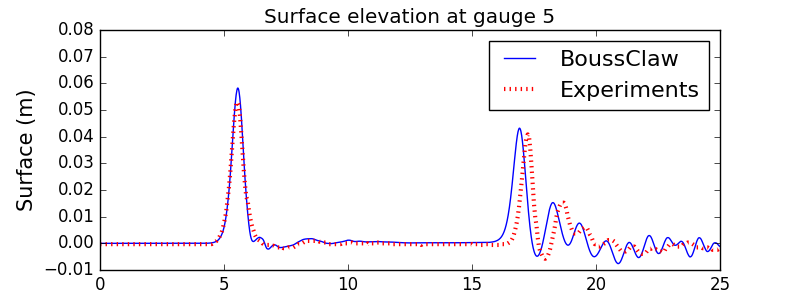
\includegraphics[width=.8\textwidth]{_fig/gauge0005fig300.png}\\
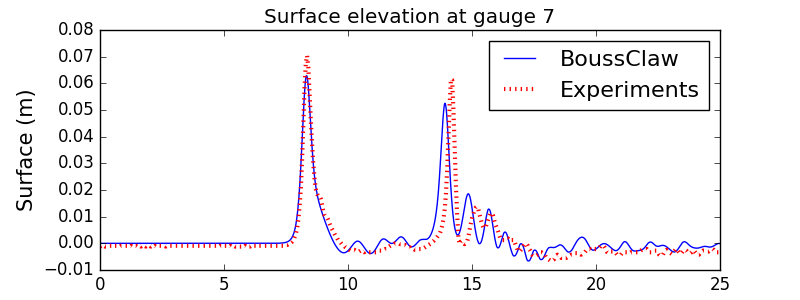
\includegraphics[width=.8\textwidth]{_fig/gauge0007fig300.png}\\
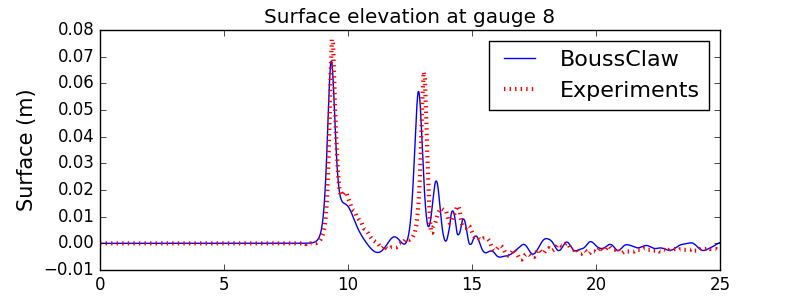
\includegraphics[width=.8\textwidth]{_fig/gauge0008fig300.png}
\caption{Comparison of \BoussClaw and experiment from \cite{chl_bp5}. Water surface elevation (m) in time (s) at gauges 5,7 and 8 for the $\alpha=0.259$ case.}
\label{fig:bp5b_gauges}
\end{figure}

%\marginpar{\footnotesize Geir: A very shallow region may yield %important frictional effects? But, surely, the wave should  break %in the shallowest region?}

\subsection{Shoaling and run-up of solitary waves}
\label{sec:shoaling_runup}


\begin{figure}[!htb]
\centering
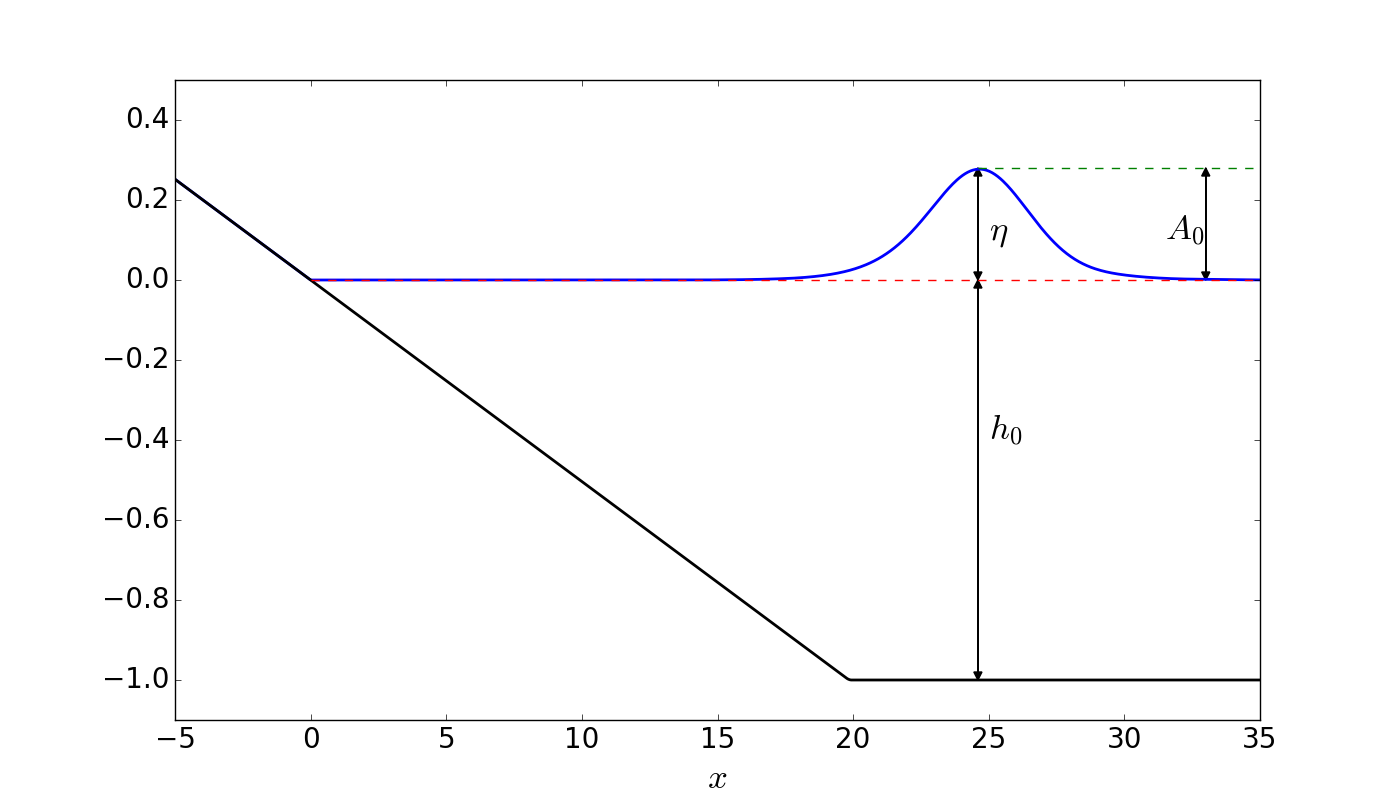
\includegraphics[width=.8\textwidth]{_fig/initial_setup.png}
\caption{Definition sketch for shoaling and runup of solitary waves. The scale on the axes is the equilibrium depth, $h_0$.}
\label{fig:init_setup}
\end{figure}
Figure \ref{fig:init_setup} shows the initial set-up for a test which 
follows the laboratory experiments by \citet{synolakis1987runup}.
The bathymetry of the wave tank is composed of a horizontal bottom, where the equilibrium depth is $h_0=0.196\m$, and 
a uniform slope as shown in Figure \ref{fig:init_setup}. 
A solitary wave of height $A_0$, hence $\alpha=A_0/h_0$, is generated at the right end of
the tank and propagates leftwards
to the beach. 

In the present section  and  throughout section \ref{sec:shoaling_breaking} we present the results using the non-dimensional coordinates 
($t^*$,$x^*$), as defined by (\ref{eq:norm_coord}) with $h_0$ as the equilibrium depth in the flat bottom region 
In  \citet{synolakis1987runup}, $t^*=0$ was defined as when the wave crest was a non-dimensional distance, $L^*$, from the toe of the slope,
where
\begin{flalign*}
& L^* = \sqrt{\frac{4}{3\alpha}} \textrm{arccosh} \left( \frac{1}{0.05} \right). &
\end{flalign*}
However, at $t^*=0$, the solitary wave has an elevation of
5\% of it maximum at the toe of the beach, meaning that the slope has
started to interact with the solitary wave. To avoid any such interaction obscuring
our analysis, we instead place the initial solitary wave using equation (\ref{eq:anal_serre}) 
with  $x^*_i=L^* + 5c$.
In this way, an incident solitary wave of amplitude $\alpha\approx 0.3$, say, has a negligible interaction with the slope when initialized. 

\subsubsection{Run-up of a non-breaking wave on a steep slope}
\label{sec:10degrunup}
On a $10^\circ$ slope an incident solitary wave of amplitude $\alpha=0.3$ will not break until the end of the draw-down phase \citep{Grilli:1997}.
Still, this may be a challenging task for Boussinesq type models \citep{Lovholt:2013a}. Run-up on a $10^\circ$ slope was investigated experimentally
by \citet{Pedersen:2013} who found a theoretical overshoot of roughly 20\% in the maximum run-up height. This was allotted to the viscous boundary layer on the beach and capillary effects. Moreover, the measurements showed that the boundary layer flow during run-up was mostly laminar, albeit indications of transition was observed in the upper part of the swash tongue close to flow reversal. Hence, it is not appropriate to employ a Manning friction term and we compare the models without any bed friction, while leaving the experiments out. 

\begin{figure}[!htb]
\centering
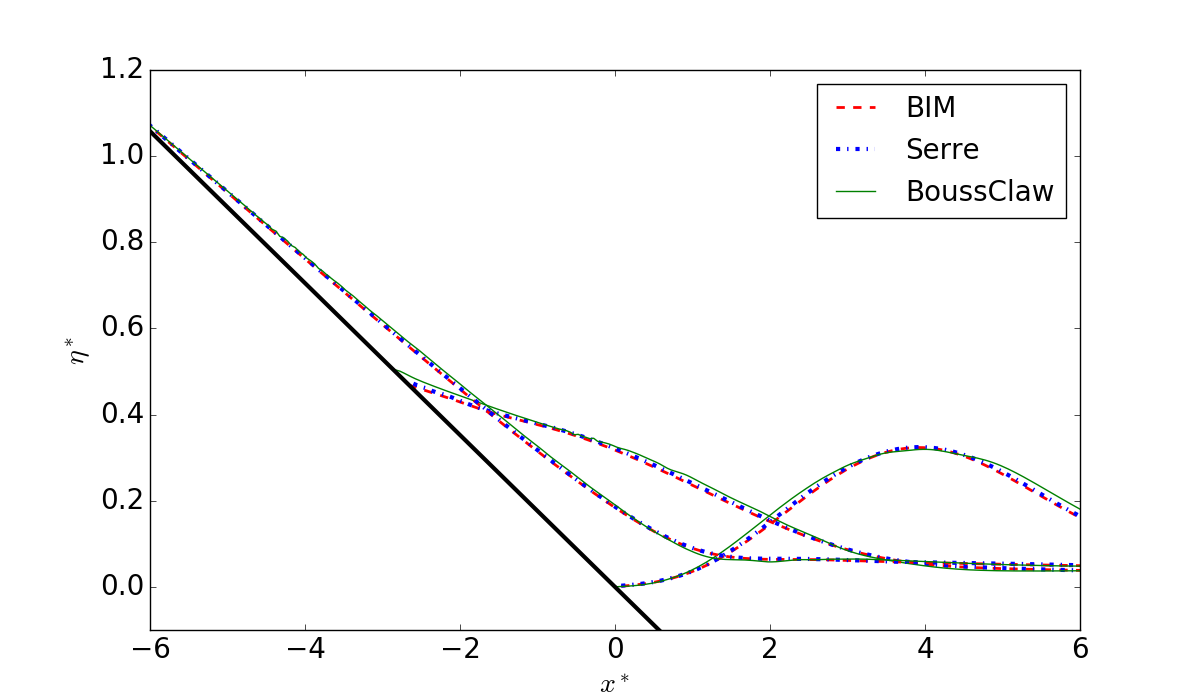
\includegraphics[height=4.6cm]{_fig/bim_serre_boussclaw_slope10}
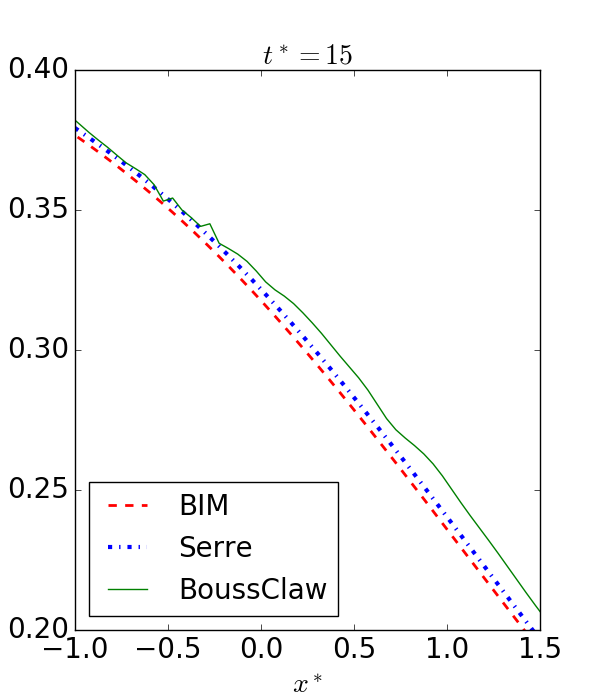
\includegraphics[height=4.6cm]{_fig/bim_serre_boussclaw_slope10_zoom}
\caption{Runup of non-breaking solitary wave ($\alpha=0.3$ and $\theta=10^\circ$). Left panel displays  surfaces from the BIM, Serre and \BoussClaw models at
	$t^* = 10,\,15,\,20$ for $\Delta x^*=0.05$. Right figure is a zoom of the results at $t^*=15$}
\label{fig:bim_serre_boussclaw_slope10}
\end{figure}

In Figure \ref{fig:bim_serre_boussclaw_slope10}, the numerical results
from BIM, Serre, and \BoussClaw are shown at $t^*=10,\, 15,\ \mathrm{and}\  20$, 
and a zoom at $t^*=15$ is shown in the right panel. 
The agreement between the dispersive models are very good. Even though the fully nonlinear Serre model follows the BIM slightly better, 
the \BoussClaw is also very close to the full potential theory. 
The small wrinkles observed on the surface 
%\todo{Check statement on wrinkles}
from the \BoussClaw (right of Figure \ref{fig:bim_serre_boussclaw_slope10}), 
are due to the switch to NLSW at the shore as discussed in section \ref{sec:10degrunup}. 
As demonstrated in Figure \ref{fig:runup_meshrefinement}, the \BoussClaw model
yields a solid grid convergence for the maximum runup height, $R^*$. 
This is in a stark contrast to observations for other models as presented in  \cite{Lovholt:2013a}.

In Figure \ref{fig:runup_slope10}, the run-up heights
are shown, and Table \ref{tab:runup_slope10} shows
the maximum run-up heights.
The NLSW model yields premature breaking (see discussion on theoretical and observed breaking in \cite{Pedersen:2013}) and a too high maximum run-up height. 
And it is observed that the NLSW model 
yields larger run-up height than the Boussinesq-type equations
for the non-breaking wave on a $10^\circ$ slope. 

\begin{figure}[!htb]
	\begin{floatrow}
		\ffigbox{%
			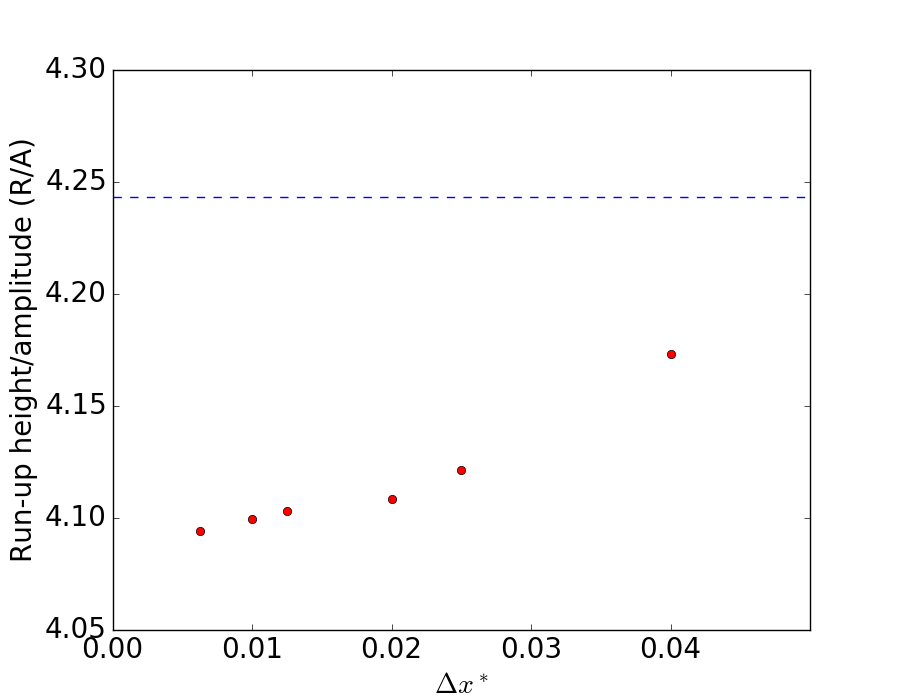
\includegraphics[width=.45\textwidth]{_fig/runup_meshrefinement}
		}{%
		\caption{Non-breaking solitary wave ($\alpha=0.3$ and $\theta=10^\circ$). Maximum run-up divided by amplitude ($R^*/\alpha$) 
			from \BoussClaw with different grid sizes.
			The dashed line is from BIM. The grid size $\Delta x^*$ is
			0.04/N and 0.025/N for $N=1,2,4$ }%
		\label{fig:runup_meshrefinement}
        }
        \ffigbox{%
        	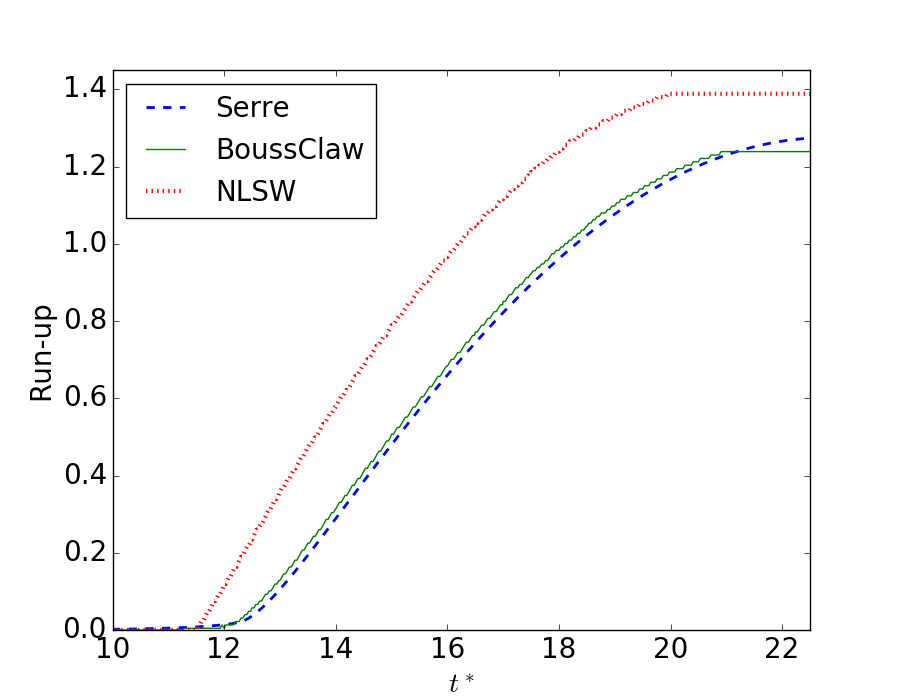
\includegraphics[width=.45\textwidth]{_fig/runup_slope10}
        }{\caption{Non-breaking solitary wave ($\alpha=0.3$ and $\theta=10^\circ$).
                  Time series for the runup height  
        	from Serre, \BoussClaw and NLSW with $\Delta x^*=0.05$.}%
        \label{fig:runup_slope10}
    }
\end{floatrow}
\end{figure}

\begin{table}[!htb]
	\begin{tabular}{c|cccc} \hline
		Model & BIM & Serre & \BoussClaw & NLSW \\ \hline
		Max. Run-up/Amp. & 4.2432 & 4.2488 & 4.0941 & 4.6561 \\
		\hline
	\end{tabular}
	\caption{Maximum run-up height divided by the incoming wave amplitude ($R^*/\alpha$) for
$\alpha=0.3$ and $\theta=10^\circ$.}
    \label{tab:runup_slope10}
\end{table}

%{\em Add figure with stages in the runup, including \BoussClaw (without the threshold), NLSW, BIM and Serre. Add figure with shoreline history until maximum runup. Add figure with convergence of BoussClaw results. Add small table with maximum runup}
 
\subsubsection{Comparison with experiments on a breaking wave}
\label{sec:wave_break}

%Depth-averaged models are not capable of handling the wave breaking unless they are modified by incorporating the energy dissipation. In this work, a breaking solitary wave will be considered on a uniform slope. For laboratory experiments, see Synolakis \{synolakis1987runup}.
From the experiments of \citet{synolakis1987runup} on runup of solitary
waves on beaches, we select the breaking case $\alpha=0.28$ 
incident on  a  $1:19.85$ slope for comparison with the \BoussClaw model. 
Experimental date is obtained at \cite{synolakis2008validation}.


%Then $t=0$ is set as soon as the peak of wave is at $x=L$.

In Figure \ref{fig:lab_bim}, the laboratory measurements
are shown with the computational results from the \BoussClaw (in Boussinesq and  NLSW mode),  the Serre and the BIM models
for $\alpha=0.28$ and a $1:19.85$ slope at $t^*=15$. 
The grid size $\Delta x^*$ is 0.05 in the following simulations
unless  otherwise is stated.
This is before the wave breaks and
the \BoussClaw, the Serre, and the  BIM model are all in good agreement with the experiments.


\begin{figure}[!htb]
\centering
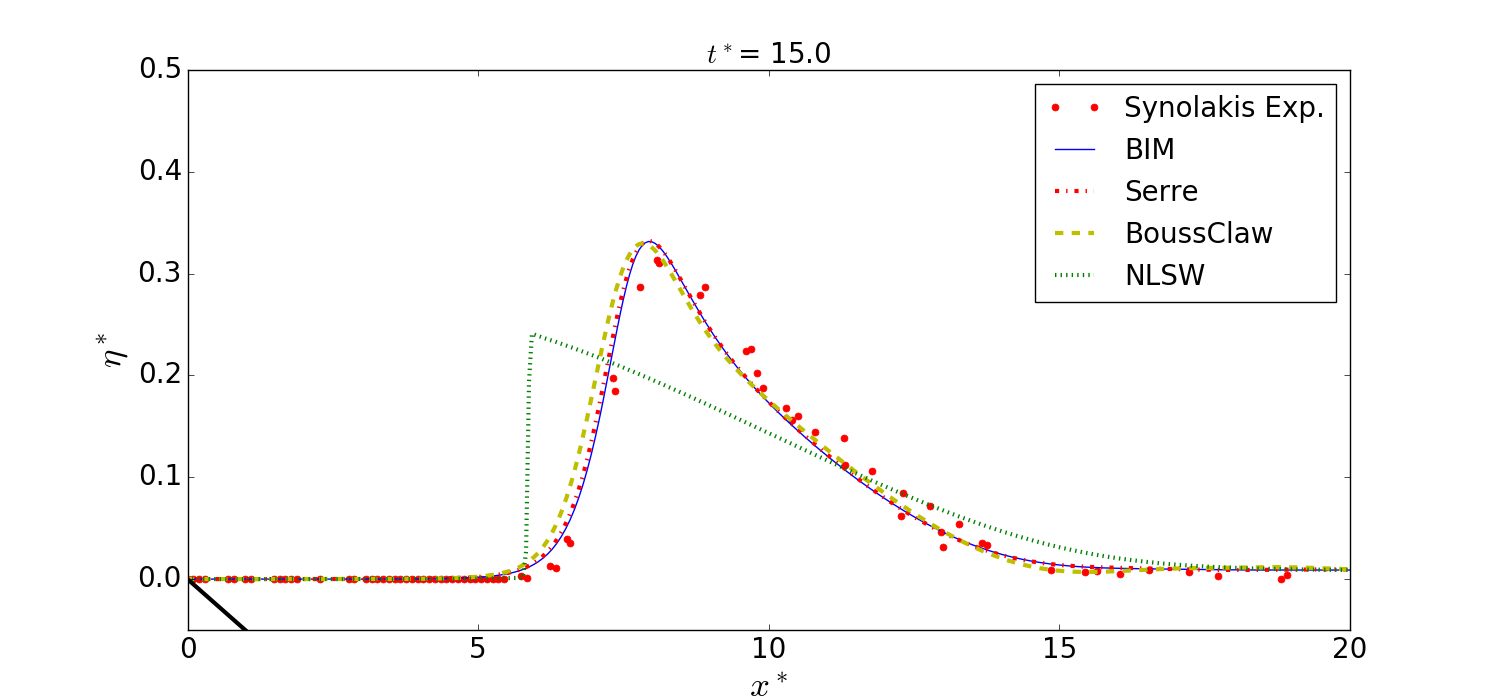
\includegraphics[width=\textwidth]{_fig/lab_bim_bouss_t15.png}
\caption{The surface elevation, $\eta^*$  as function of $x^*$ at $t^*=15$ from the laboratory experiments \citep{synolakis1987runup} ($\alpha=0.28$, slope $1:19.85$), the BIM, the Serre, the \BoussClaw and the NLSW models.}
\label{fig:lab_bim}
\end{figure}
%\todo{Add Serre results in figure and give web adress for data as reference}
%\marginpar{\footnotesize What is the result of Titov and Synolakis?} 
%and the undisturbed depth is $h=0.206$ m. 

The ratio of amplitude to depth, $A^*/h^*$ ($A^*$ is the maximum value of $\eta^*$ and $h^*$ is the equilibrium depth at the
corresponding location), 
is about $2$ at the point of breaking.
The potential flow model cannot be run much beyond the
breaking points (until the attachment of the plunger only) and 
gives no information on the following bore propagation.
In figure \ref{fig:BoussClaw_runup} we have compared
the experimental data with the \BoussClaw model 
of $C_d^* = 0$ and $0.03$.

The agreement is good and the introduction of bed-friction 
even seem to match the truncated swash tongue of the experiments well. However, this may be a coincidence. 
Even though the  wave has broken and some irregular flow features are introduced thereby, we have no evidence of the flow state being
anywhere near turbulent, which is required for a quadratic bottom resistance to be appropriate. 
Capillary effects and 
experimental errors may also affect the comparison
as observed by \cite{Pedersen:2013}.

\begin{figure}[tbh!]
	\centering
	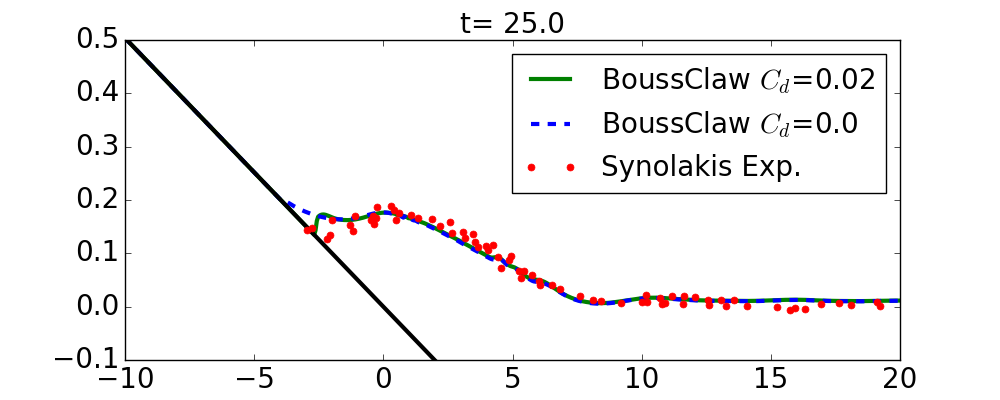
\includegraphics[width=.8\textwidth]{_fig/BoussClaw_lab_Cd_t25}\\
	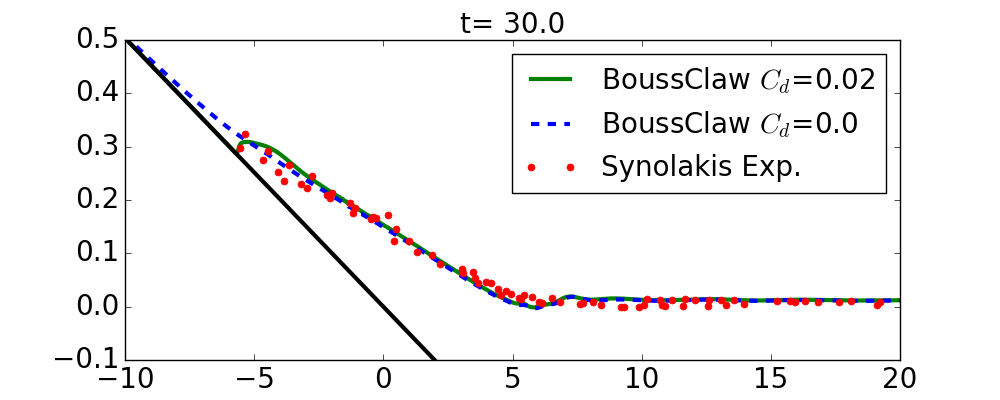
\includegraphics[width=.8\textwidth]{_fig/BoussClaw_lab_Cd_t30}
	\caption{The surface elevation $\eta^*$ as function of $x^*$ at $t^*=25,\,30$ for the breaking case ($\alpha=0.28$ and a $1:19.85$ slope).
       Experiments and BoussClaw results with and without bottom drag are
        included. 
		The resolution in the model is $\Delta x^* = 0.05$.}
	\label{fig:BoussClaw_runup}
\end{figure}

In Figure \ref{fig:runup_slope_1_20} and Table \ref{tab:max_runup_1_20},
we show the run-up height in time and the maximum run-up height respectively.
Unlike what was observed for $\theta=10^\circ$, the NLSW model
reduces the run up height. 
The opposite behavior for the two may be 
explained by two competing effects of dispersion. 
First, for a non-breaking wave the omission of non-hydrostatic effects 
lead to an excessive 
steepening of the wave front which implies higher run-up. 
On the other hand, 
the premature breaking dissipates energy and will reduce run-up heights. 
For the steeper slope, 
there is insufficient time for the second effect to fully 
counterbalance the first. 
For the gentler slope the early onset of breaking
in the NLSW model, at a long distance form the shoreline, causes a large 
dissipation which dominates over the first effects.

In addition to affecting the runup a non-zero $C_d$ will delay, or even inhibit the withdrawal.
A detailed discussion of such effects is outside the scope of the present article and we refer instead to 
a profound investigation in \cite{antuono2012role}.  
%\todo{Geir: But, Li and Raichlen obtained a smaller runup height; Manning friction ? Check.}

\begin{figure}[!htb]
	\centering
			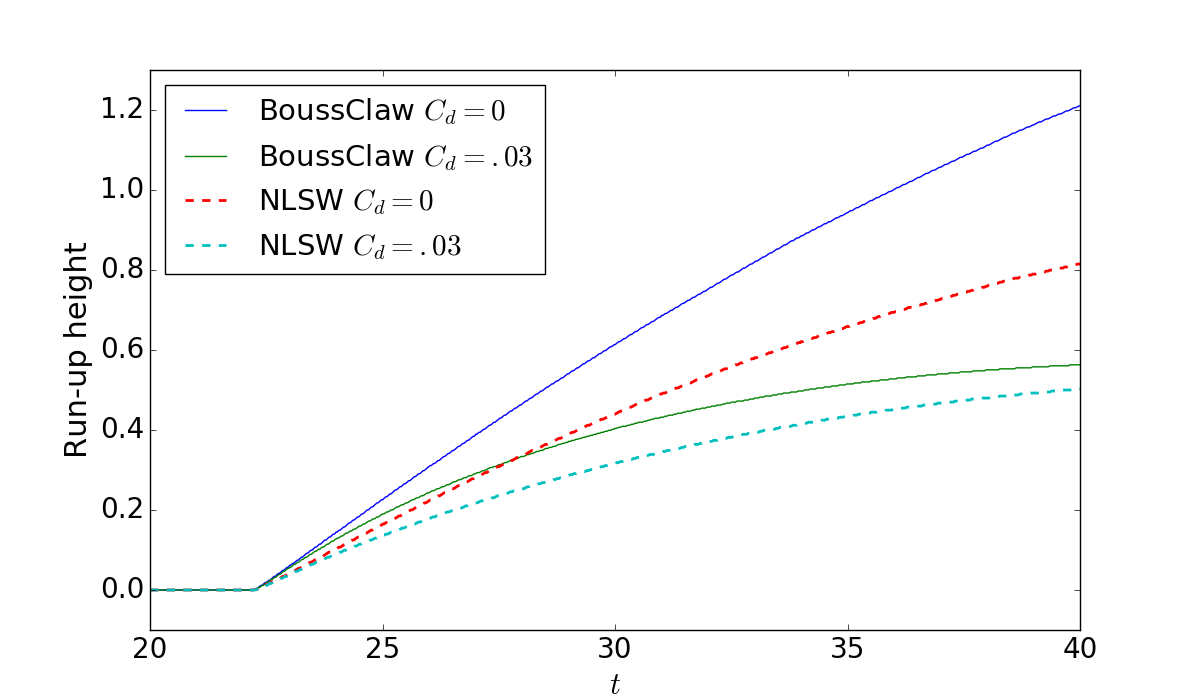
\includegraphics[width=.8\textwidth]{_fig/runup_slope_1_20}
		\caption{Dimensionless shoreline elevation for the breaking case ($\alpha=0.28$ and a $1:19.85$ slope) computed by \BoussClaw 
			(without $\epsilon_B$) and NLSW with different $C_d^*$.}
		\label{fig:runup_slope_1_20}
\end{figure}

\begin{table}
		\begin{tabular}{cccccc} \hline
			           $C_d^*$ & 0 & 0.01 & 0.02 & 0.03 &  \\ \hline
			\BoussClaw (without $\epsilon_B$)& 1.634 & 0.921 & 0.691 & 0.576  &  \\ 
			\BoussClaw ($\epsilon_B=0.8$)& 1.193 & 0.848 & 0.696 & 0.608 &  \\
			NLSW & 0.936 & 0.702 & 0.596 & 0.528 &  \\
			\hline
			Experiment  & & & & & 0.551 \\
			\hline
		\end{tabular}
	\caption{Maximum run-up height, $R^*$, for a solitary wave of amplitude $\alpha=0.28$ incident on  a $1:19.85$ slope.}%
	\label{tab:max_runup_1_20}
\end{table}

%The computation of BIM can not proceed further after $t=19.2$ because of the singularity.

%One of the main reasons is to exclude the effect of the bottom friction. Without appropriate inclusion of the friction forces, the numerical results will not yield comparable results with the experiments. When different numerical models are compared, however, it is difficult to distinguish the friction errors from the modeling errors. Therefore, the numerical solution of BIM without any friction is considered as a solution.

%Figure \ref{fig:sw_timeseries} and \ref{fig:bous_timeseries} show the computational results from depth-averaged models, and both models do not capture the wave breaking properly.
%In Figure \ref{fig:bous_timeseries}, the numerical results from the \BoussClaw are given, the amplitude of the incoming wave continues to increase and the wave does not break. 

%\begin{figure}[!htb]
%\centering
%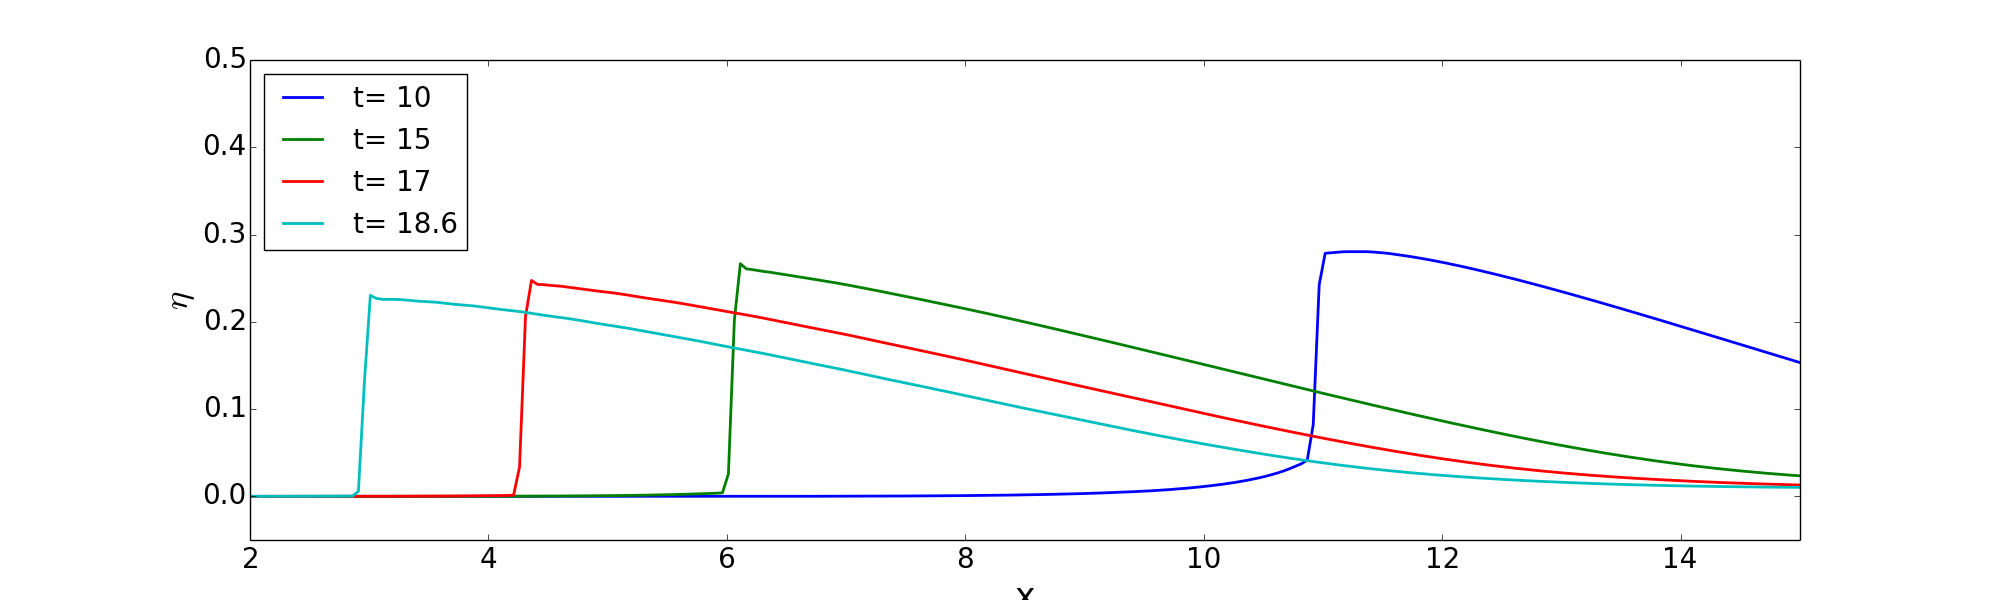
\includegraphics[width=\textwidth]{_fig/sw_dx05_time_series.png}
%\caption{Computational results from NLSW at $t=10,15,17$ and $18.6$.}
%\label{fig:sw_timeseries}
%\end{figure}

%\begin{figure}[!htb]
%\centering
%\includegraphics[width=\textwidth]{_fig/bous_dx025_time_series.png}
%\caption{Computational results from \BoussClaw 
%at $t= 5,9,13,17$ and $20$ s.  }
%\label{fig:bous_timeseries}
%\end{figure}

\section{Shoaling and breaking phenomena}
\label{sec:shoaling_breaking}

\subsection{Shoaling until breaking}
\label{sec:num_shoaling}
\citet{wei1995fully} made computations of pre-breaking solitary wave shoaling using
 their fully nonlinear extension of Nwogu's model, a full potential 
theory, and the weakly nonlinear version of Nwogu's model.
They found that the fully nonlinear Boussinesq equations were superior to those of Nwogu in the later stages of the shoaling.
In this subsection we will do a similar comparison for our models on the $1:19.85$ slope which was not included in the reference. Our fully nonlinear Boussinesq model is different from that of the references, as it is a Serre type model with the depth averaged velocity as primary unknown, 
and our  \BoussClaw model is not fully nonlinear. Hence, it is imperative
to test the shoaling properties, particularly for the latter model.   
 
We use the set-up described in section \ref{sec:wave_break} for the Boussinesq modeling of solitary waves on a slope. 
The \BoussClaw simulations are compared
with those of other Boussinesq solvers, namely
 \textsc{Funwave} \citep{shi2012high}, \textsc{GloBouss} \citep{lovholt2010coupling} and the Serre type formulation \citep{Lovholt:2013a}.
As noted above, 
the original Serre's equations are enhanced by adding the same kind of dispersion correction terms as are used in 
(\ref{eq:madsen_momx}). 


\begin{figure}[tbh!]
\centering
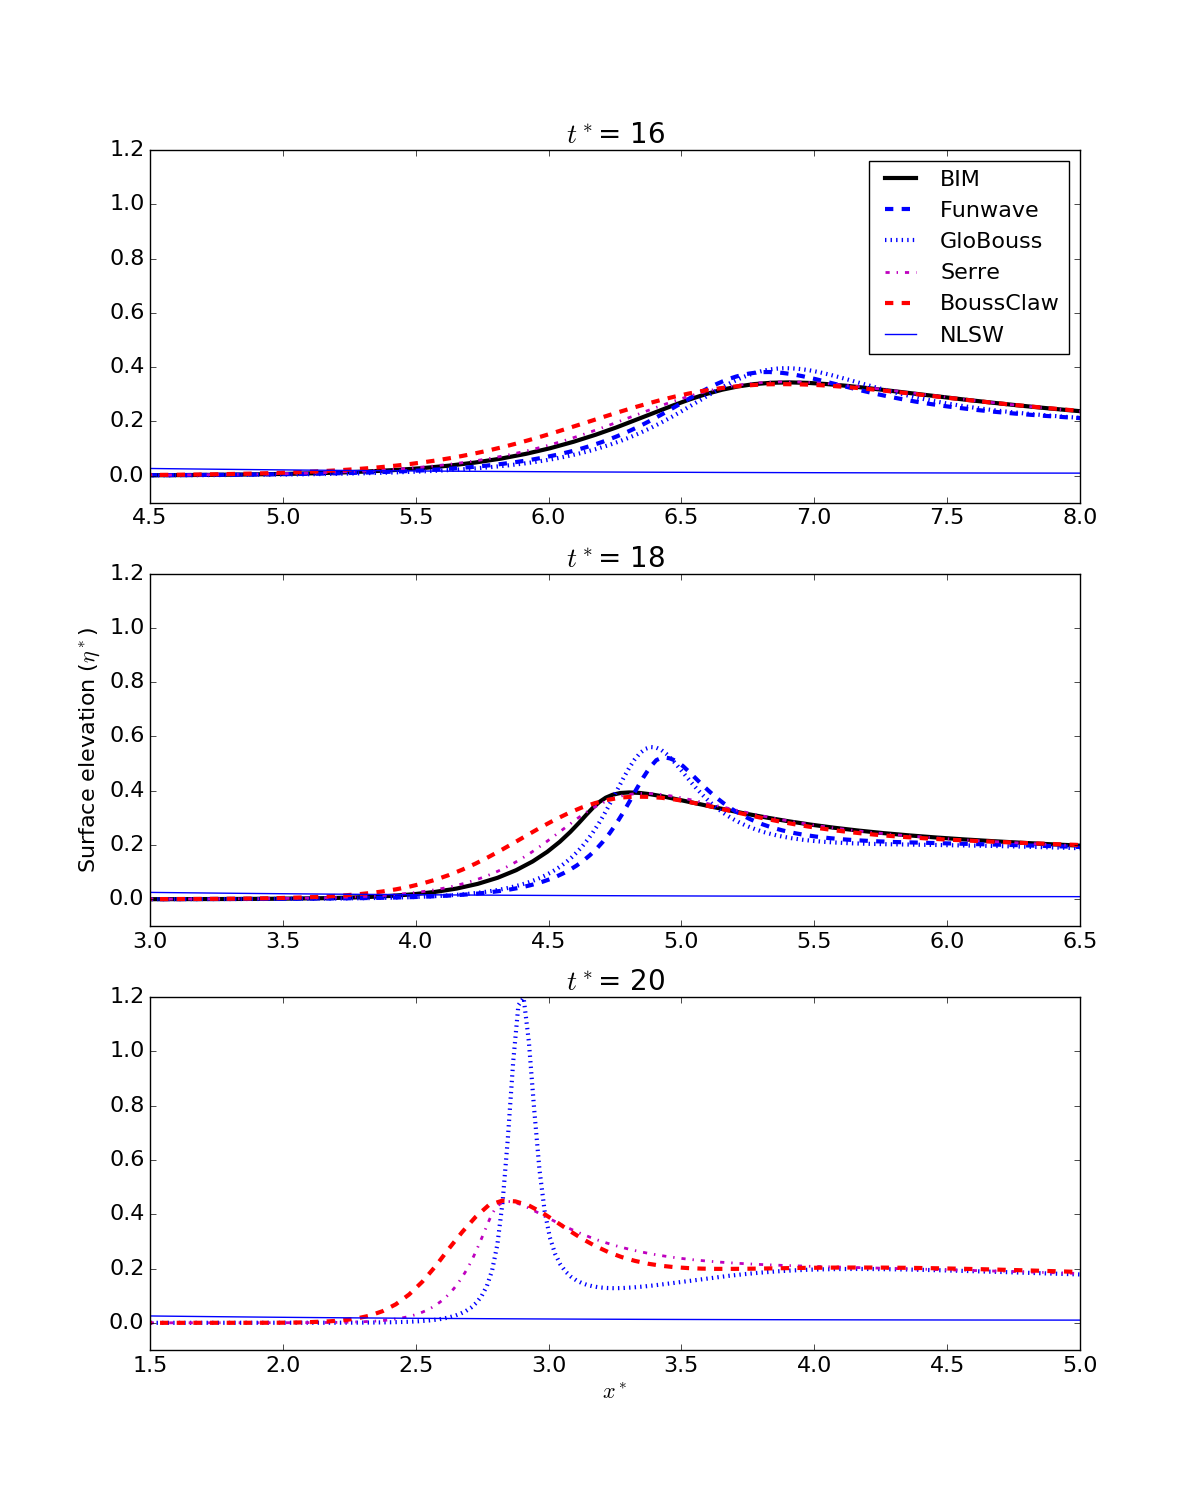
\includegraphics[width=.9\textwidth]{_fig/bim_boussclaw_fun_glob.png}
\caption{Evolution of $\eta^*$ for $\alpha=0.28$ and a $1:19.85$ slope. 
Surfaces from the BIM, Serre, \textsc{GloBouss}, \BoussClaw
and \textsc{Funwave} models at $t^* = 16,\, 18,\ 20$ are included.
The \BoussClaw model is used with B=$1/15$,
and the Peregrine's equations are used for \textsc{GloBouss}.}
\label{fig:bim_boussclaw_fun}
\end{figure}

In Figure \ref{fig:bim_boussclaw_fun} surfaces from the different
wave models are shown at selected times. 
The \BoussClawt model is run without the switch to the NLSW equations at $\epsilon_B=0.8$ and with the dispersion parameter $B=1/15$. However, the results for  $B=0$
are rather similar to those for $B=1/15$ in this case. 
At $t^*=16$, the computational results
from all the Boussinesq-type equations are similar.
The NLSW model, on the other hand, yields premature breaking 
causing a too low amplitude. 
At $t^*=18$, some discrepancies are observed. The models  
can be split into two groups; 
\textsc{GloBouss} and \textsc{Funwave} 
are similar, while the \BoussClaw
and the Serre results are similar. 
The wave front from the 
\BoussClaw model is somewhat more advanced towqard  the beach than that from the BIM model.
Still, the results from the Serre and \BoussClaw models are clearly
closer to those of the BIM model, than those from the other group. 
Especially, the wave amplitudes are well  determined by the \BoussClaw
and the Serre  models.
The wave amplitudes computed by the \textsc{GloBouss} and \textsc{Funwave} models, on the other hand,
are more than 33 \% 
larger than those from the BIM model at $t^*=18$.
The wave amplitude continues to increase in the
\textsc{GloBouss} simulations,
and the difference from the \BoussClaw result 
becomes larger at $t^*=20$. At the $t^*=20$ there are no results from the BIM model as  the wave has broken.
Our observations on model performance during shoaling are in line with those of \citet{wei1995fully}.
 
\subsection{Wave breaking and run-up}
\label{sec:discuss_breaking}
In the BIM model we may identify the onset of breaking as the instant when we first observe a vertical slope at the wave front.
For an incident amplitude of $\alpha=0.28$ on a $1:19.85$ slope,
a vertical wave front is observed at $x^*=4.09$ and $t^*=18.6$ with $A^*/h^*=2.01$.
When the crest in the \BoussClaw simulation reaches $x^*=4.09$, 
we find $A^*/h^*=1.97$.
The threshold value $\epsilon_B=0.8$ (see sec.~\ref{sec_add_num})
is  reached already at $t^*=14.9$
when the peak of the wave is at $x^*=8.03$.
In the following, we explore the wave evolution with and without
the switch to the NLSW equations at this threshold.


In Figure \ref{fig:boussclaw_th08}, snapshots are shown for
$t^*$ equal to $20$, $25$ and $30$ of the solutions from \BoussClaw and NLSW
with the Manning coefficient $C_d^*=0.03$.
At $t^*=20$ the simulation with $\epsilon_B=0.8$ has already been in NLSW mode for $5$ time units and the difference in the wave height 
from the full Boussinesq simulation is significant. In fact, the threshold solution is closer to the NLSW solution.

\begin{figure}[tbh!]
	\centering
	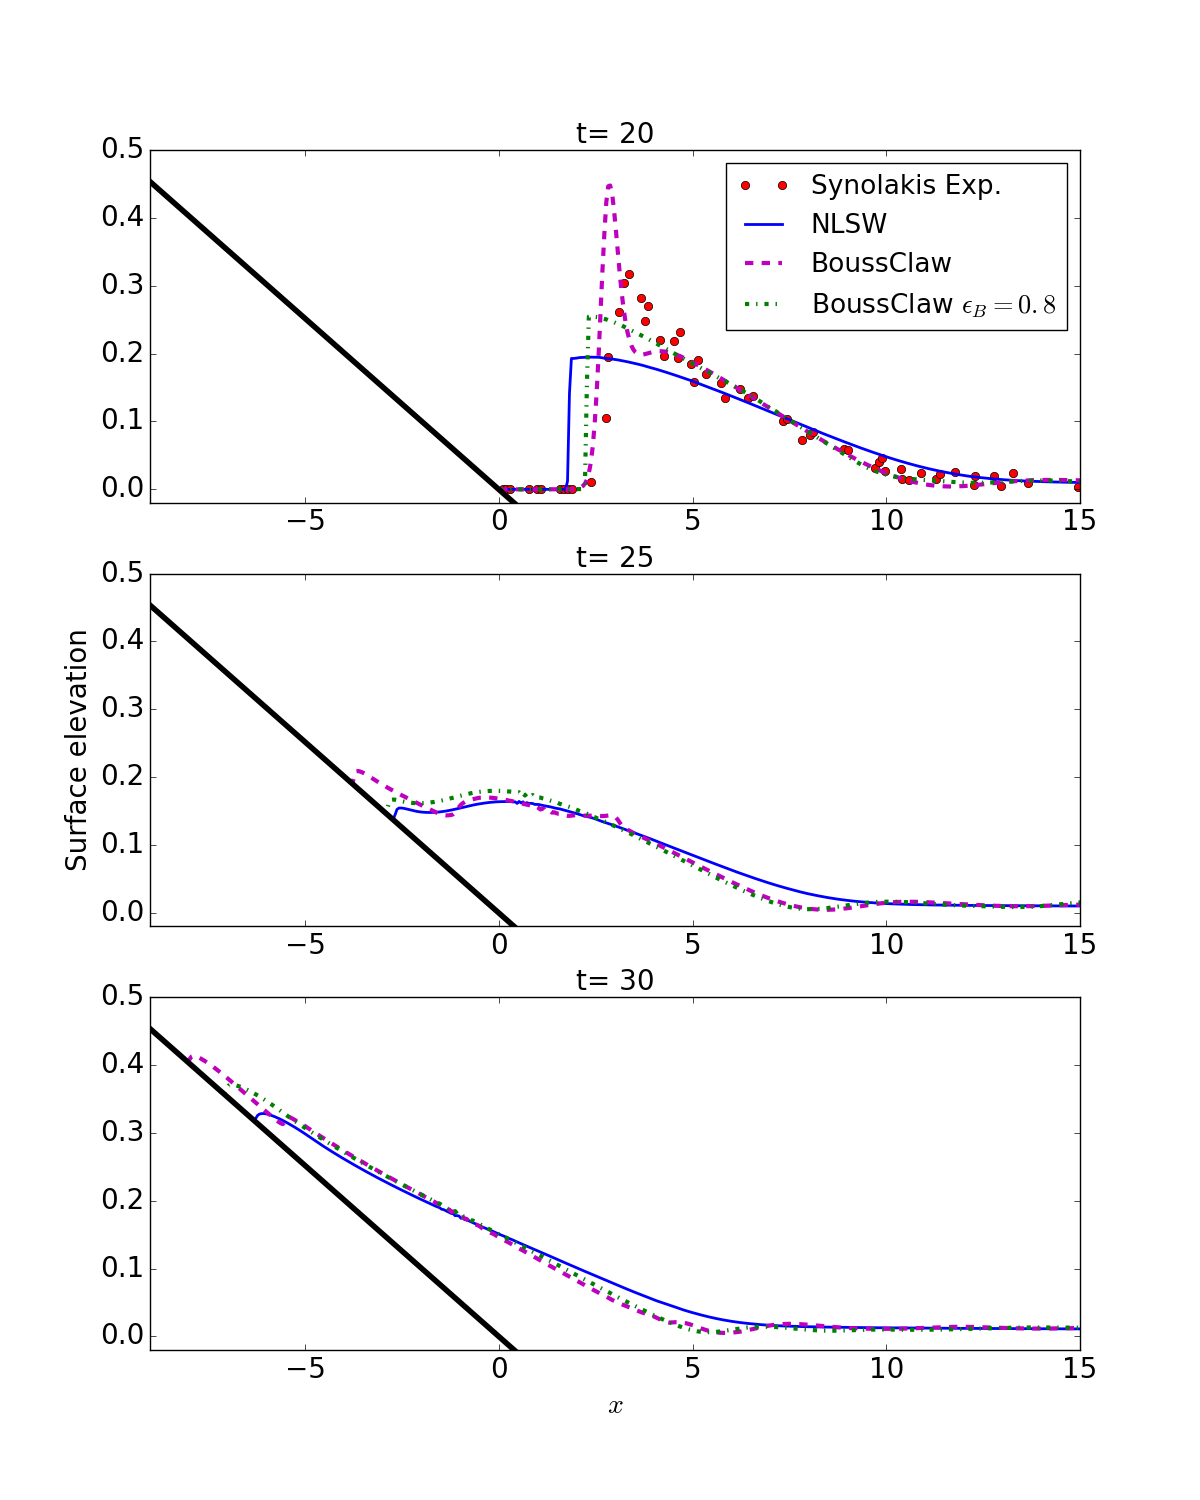
\includegraphics[width=.75\textwidth]{_fig/bim_boussclaw_etaB8}
	\caption{Breaking case ($\alpha=0.28$ and a $1:19.85$ slope).
                 Comparison of $\eta^*$ from  \BoussClaw and NLSW 
with $\epsilon_B=0.8$ and $\Delta x^* = 0.05$ at $t^*$ = $20$, $25$ and $30$. Friction forces have been added with $C_d^*=0.03$ in all simulations.}
	\label{fig:boussclaw_th08}
\end{figure}

At $t^*=25$ and $t^*=30$, the wave is running up the slope, 
and the difference in the swash tongue is relatively small. 

Other measures of nonlinearity than $\epsilon_B$ may be used for model decisions 
\citep{lynett2006nearshore,matsuyama2007study}. Figure \ref{fig:wave_break_criteria} shows 
$\epsilon_B$, $u^*/\sqrt{H^*}$ ($H^*$ is the total, dimensionless, flow depth) and the maximum frontal angle 
as a function of the crest location.
When the the BIM model yields a vertical front at $x^*=4.09$, 
we obtain $u^*/\sqrt{H^*} = 1.034$ and a maximum surface slope angle of $39.1^\circ$. 
%\todo{OK?}
For the present case this might indicate 
that the value of $u^*/\sqrt{H^*}$\marginpar{Is it the maximum or value at the peak?}
 at the peak surpassing unity or the slope angle surpassing  
$30^\circ$ may be sounder criteria for identifying breaking than $\epsilon_B>0.8$.
 
\begin{figure}[tbh!]
\centering
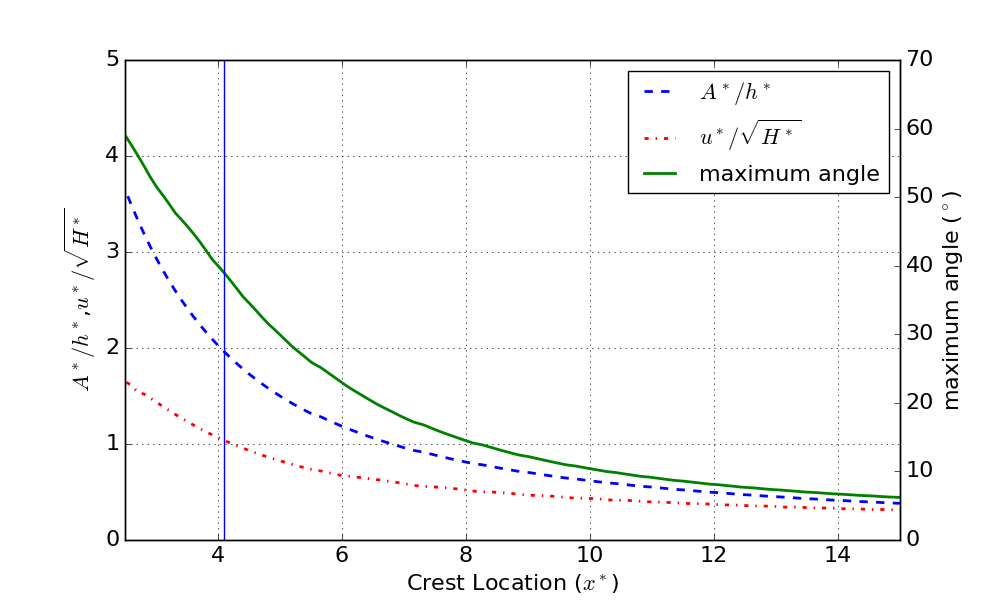
\includegraphics[width=.7\textwidth]{_fig/wave_break}
\caption{Plot of $A^*/h^*$, $u^*/\sqrt{H^*}$ and maximum angle of waves vs. crest location. 
The vertical line indicates where the BIM model yields breaking ($x^*=4.09$). }
\label{fig:wave_break_criteria}
\end{figure}

\subsection{Wave Energy}
\label{sec:wave_energy}
The gross wave energies  
for the shallow water equations and Boussinesq equations
are $E^*_0$ and $E^*_0+E^*_1$  respectively, as explained in \ref{append:energy}.
As stated in section \ref{sec:sol_prop} they are made dimensionless by the factor $E_c=\rho g h_0^3$. 
In Figure \ref{fig:energy_boussclaw_swe} the energy densities are depicted as 
functions of the crest location, $x^*_c$. 
In the left panel 
we observe that the $E^*_0$ is nearly constant 
for the shallow water equations until a shock is formed around $x^*_c=13$.
Thereafter, energy is quickly dissipated. For the \BoussClaw simulations $E^*_0$
increases slightly, but noticeably, during shoaling, indicating that $E^*_1$ needs to be accounted for.
In  the \BoussClaw simulation with no threshold (right panel) 
$E^*_0+E^*_1$ is nearly constant when the wave propagates in constant depth. 
On the deeper parts of the slope there is first a small increase, then a
very moderate reduction. Presumably, the increase is  due to the absence of strict energy  conservation in the Boussinesq equations. 
Close to the shoreline this tiny increase is then dominated by a stronger, but still mild, energy dissipation.
When the threshold $\epsilon_B=0.8$ is invoked there is no difference from the full Boussinesq solution until the threshold is reached for  $x^*_c=x^*_B=8.03$. 
After  $x^*_c=x^*_B$  
the hydrostatic energy measure, $E^*_0$, is the most appropriate for this case.
The energy  drops momentarily due to the change of energy formula, then remains constant until the wave breaks ($x^*_c$ around 6), after which a strong dissipation ensues.

In this case the dissipation is due to a single shock. The dissipation rate per width, $D_{th}$, may then be
approximated as \citep{tissier2011serre} 
\begin{flalign}
	D^*_{th} = \frac{1}{4}
	\left( \frac{2h^* + d^*}{2h^*(h^*+d^*)} \right)^{1/2}
	(d^*)^3,
\label{eq:energy_dissipation}
\end{flalign}
where $d^*$ is the shock height, which, for a fully developed bore, corresponds to maximum $\eta^*$ ($A^*$) in our case,
and $h^*$ is 
the undisturbed water depth. The rate $D^*_{th}$ has been made dimensionless by the factor $E_c\sqrt{\frac{g}{h_0}}$, where $E_c$ is given above.
In figure \ref{fig:energy_decay} 
we observe that the dissipation rates of the models has a build-up, before the 
shock is fully developed, 
and then agree well with  formula (\ref{eq:energy_dissipation}).
Moreover, due to larger shock heights the \BoussClawt($\epsilon_B=0.8$) dissipation rate is much larger than that of the NLSW model, when the wave finally has broken.
This reduces the difference between the models to some extent. 
It is obvious that the NLSW model in this case is severely inaccurate, while 
it is more difficult to assess the \BoussClaw 
with and without the switch to the NLSW.

\begin{figure}[tbh!]
	\centering
	\begin{subfigure}[t]{0.45\textwidth}
		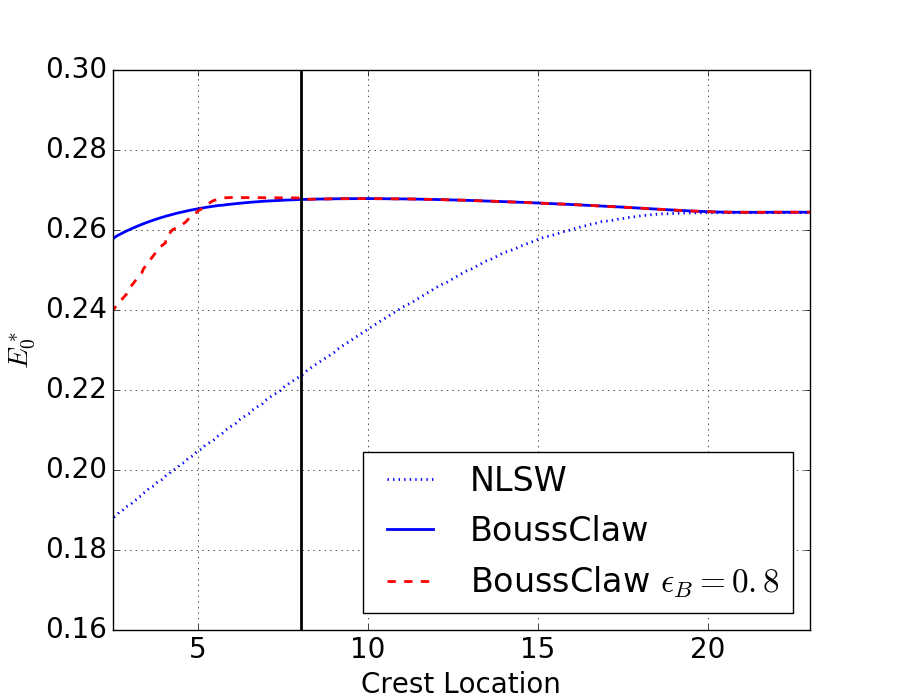
\includegraphics[width=\textwidth]{_fig/e0_boussclaw_eb08.png}
		\caption{}
		\label{fig:e0_boussclaw_eb08}
	\end{subfigure}
	\begin{subfigure}[t]{0.45\textwidth}
		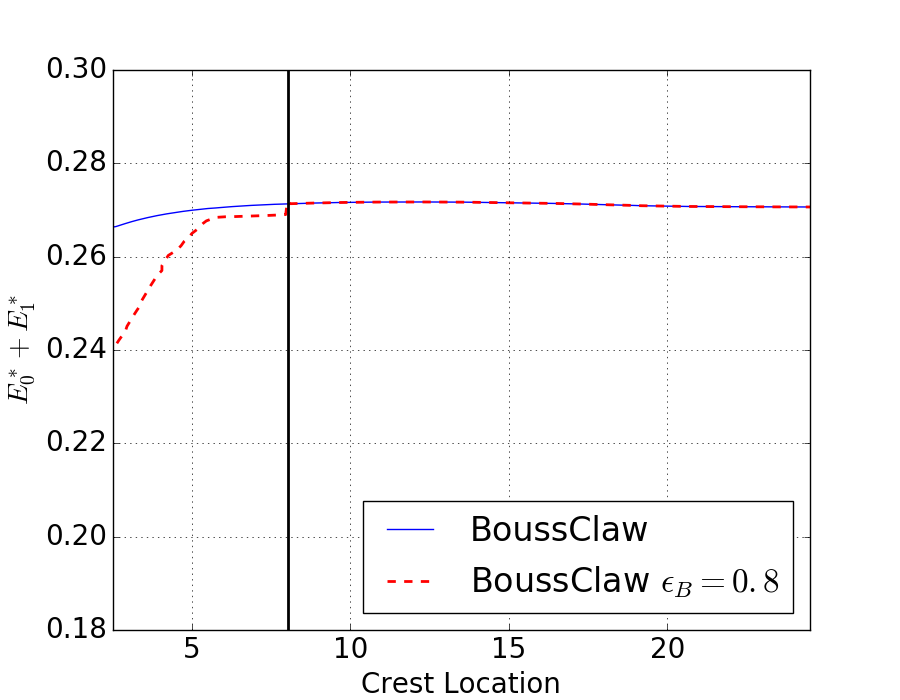
\includegraphics[width=\textwidth]{_fig/e1_boussclaw_eb08.png}
		\caption{}
		\label{fig:e1_boussclaw_eb08}
	\end{subfigure}
	\caption{Wave energy ($\alpha=0.28$, slope $1:19.85$) as function of crest position. The vertical line is at $x^*=8.03227$  where $\epsilon_B=0.8$. (a): $E^*_0$. (b): Solid line is $E^*_0+E^*_1$ of \BoussClaw without $\epsilon_B$. With $\epsilon_B=0.8$, $E^*_0$ is shown in dashed line after the threshold is reached.
 }
	\label{fig:energy_boussclaw_swe}
\end{figure}

\begin{figure}[htb!]
\centering
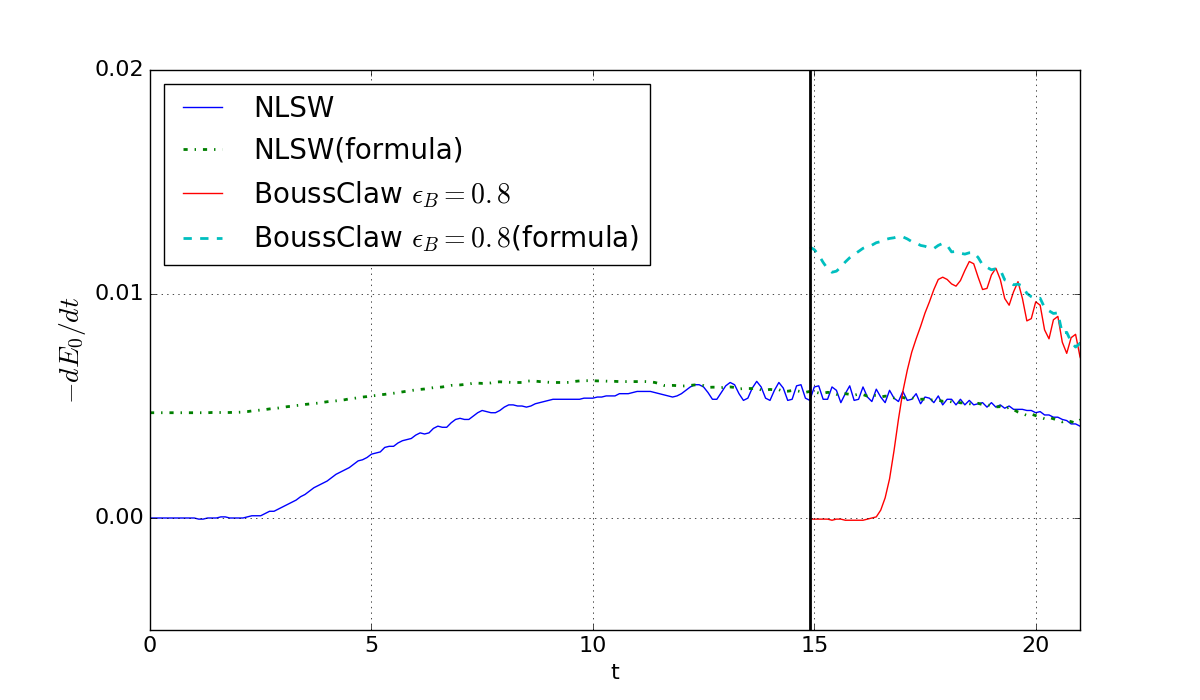
\includegraphics[width=0.8\linewidth]{_fig/energy_decay}
\caption{Dimensionless energy dissipation rates for $\alpha=0.28$ and a $1:19.85$ slope. The label ``formula'' represents (\ref{eq:energy_dissipation}) inserted the wave heights from the numerical simulations.
	\BoussClaw with $\epsilon_B=0.8$ switches to the NLSW
	at $t^*=14.9.$ }
\label{fig:energy_decay}
\end{figure}

The onset of the dissipation in the threshold model comes slightly before the a vertical front is observed in the BIM solution $x^*_c=4.09$. This may point to a too early and strong dissipation. On the other hand, the Boussinesq solution without the threshold most likely
yields too little dissipation. In this context we remark that the experimental data in
the upper panel of figure \ref{fig:boussclaw_th08} apparently fall between the \BoussClaw results with and 
without the $\epsilon_B$ threshold, even though there is scatter in the experimental 
surface. 
The last step of the procedure in section \ref{sec:Num_scheme}, which
deals with the dispersion, increases the wave front width to  the order of
the local depth and thus reduces the dissipation 
of the next TVD step. This effect of the dispersion terms may be inferred from, for instance, the Green function of Helmholtz type equations as outlined in \cite{Glimsdal:2004}, section 3.1.1. Still, the \BoussClaw model, without the threshold, is stable during 
both the last part of shoaling and during runup, even for refined grids. This contrasts
the non-dissipative Serre model which may be run beyond $x^*_c=4$, without the strong artificial amplification of the Peregrine type models, but breaks down when the wave reaches the shoreline (results not shown). Hence, \BoussClawt, without the switch to the NLSW equation at
$\epsilon_B=0.8$, may be a good model for gently spilling breakers.



\section{Concluding remarks}
\label{sec:conclusion}
The \BoussClaw extension to the \textsc{GeoClaw} package includes Boussinesq type equations
and resembles much used general purpose models such as \textsc{Funwave-TVD} and
\textsc{Coulwave-TVD}, but is based on a different and somewhat  simpler 
set of governing equations, as well as a slightly different numerical scheme. 
Comparisons with other models as well as experiments are good. Moreover,
the model does not display the vulnerability to instabilities for 
strong nonlinearities in shallow water
as is observed for some fully nonlinear Boussinesq models \citep{Lovholt:2013a}. 

The experiments of \citet{synolakis1987runup} and a full potential reference model
 enabled us to
assess a set of different long wave models, and \BoussClaw in particular. Using the potential  model, we were able to assess in detail the pre-breaking behavior of the models,
and to identify the point of breaking accurately. 
First, we found that by using standard NLSW models,
the point of breaking will be located too far offshore and that the resulting dissipation 
artificially check the amplification. Standard Boussinesq equations, like the 
so called Peregrine variant, yield marked over-amplification even before the potential theory predicts breaking and they eventually produce completely erroneous wave shape as well as height.
The fully nonlinear, non-dissipative model of the Serre type, on the other hand, follows full potential theory very well up to the point of potential-model breaking and avoid severe over-amplification and shape distortion also in the following evolution, until it breaks down at the shoreline. For the pre-breaking part, this is in agreement with earlier investigations of equations of the Nwogu/Wei type \citep{Wei95} and shows that
the combined effects of nonlinearities and dispersion influence the solution markedly, when accumulated to the point
of breaking. 
However, herein we find also a very good pre-breaking performance of 
the \BoussClaw Boussinesq equations 
where only some nonlinearity is retained in the dispersion. 
This suggest that the practice of retaining full nonlinearity 
in Boussinesq shoaling/runup models 
may be relaxed, especially when the switch to the NLSW equations are invoked. 
%when the wave-height to depth ratio surpasses a threshold of $0.8$. 
This may help reducing stability problems 
that are observed for fully nonlinear Boussinesq equations \citep{Lovholt:2013a}.
    
A current practice has evolved in which the Boussinesq terms are omitted near shore through the $A/h>0.8$ threshold criterion, inspired by the maximum height of a non-breaking 
undular bore. 
In an example presented herein, we investigated the near shore propagation over a relatively gentle shelf of $1:19.85$ slope,
and in this case the actual onset of breaking occurred for $A/h \approx 2$, which is significantly later
than what would be predicted by the threshold.  
Hence, a  threshold criterion may lead to an erroneous breaking point as well as an 
inaccurate description of the later stages of the shoaling.
It is noted that the artificial effect discovered would depend on the slope, 
and a $0.8$ threshold may well work better on a much gentler slope as it is primarily derived based on 
solitary wave properties in constant depth. On the other hand, $1:19.85$ slope is already quite gentle,
and the offset between the reference solution and Boussinesq models using this criteria may
be even more pronounced for steeper slopes.

\appendix

\section{Stability of the hybrid scheme}
\label{append:stab}
It is difficult to analyze the numerical stability for  our full Boussinesq
equations. 
To obtain some insight in the  stability of the proposed hybrid numerical scheme,
we thus consider a closely related, but simpler, equation, namely the 
linearized Benjamin-Bona-Mahony (BBM)
equation (\cite{benjamin1972model}) 
\begin{align}
u_t + c u_x = \frac{h^2}{6}u_{txx},
\label{eq:basic_1}
\end{align}
where $c=\sqrt{gh}$.
This equation describes weakly dispersive, uni-directional waves in constant
depth. The equation replaces the momentum equation, whereas no separate
continuity equation is involved.

Following the steps of section \ref{sec:Num_scheme},
we rearrange 
the equation (\ref{eq:basic_1}) as
\begin{align}
(I-D)(u_t + c u_x) +Du_x = 0, \label{eq:basic_2}
\end{align}
where $D=\frac{h^2}{6}\partial_x^2$.
The first step of  hybrid scheme for  this equation is integration of
 the advection equation
\begin{align}
u_t + c u_x = 0,
\label{eq:append_advec}
\end{align}
by the finite volume method. 
Then the Runge-Kutta  method is applied to,
\begin{align}
(1-D)u_t + cDu_x = 0.
\label{eq:append_mom_fdm}
\end{align}
which is the counterpart to  (\ref{eq:hybrid_mom_fdm}).

If we use the centered spatial difference approximation of $O(\Delta x^2)$
accuracy on a regular grid we may employ a standard von Neumann analysis where we calculate the growth of an harmonic mode over a single time step.
Expressing the coefficients of the velocity array before the time step as  $u_j= e^{i\xi j \Delta x}$ we then replace the coefficient of $\textbf{M}^k$, defined in section \ref{sec:Num_scheme}, 
by $M_j^k=U_j^k= g^ke^{i\xi j \Delta x}$, 
where $k$ is 1, 2, 3, 4 or +. Correspondingly, the coefficients of the $\mathbf{S}^k$ array, which contains auxiliary,  nodal values for $u_t$,  is
expressed $(S_j^k)= s^k e^{i\xi j \Delta x}$. 

The stability  of the first step, (\ref{eq:append_advec}),  is assured by the standard CFL criterion
\[\frac{c\Delta t}{\Delta x} <1.\]
If we instead solve the NLSW equations, as in \BoussClawt, $c$ must be replaced by the nonlinear characteristic velocity, which may lead to a more strict criterion. However, the method employed in the first step is not suited for a von Neumann stability analysis and we thus apply this technique to the second step only. 
 Hence, we may put $g^1$ to unity, but it is preferable to retain it in the calculations. 
The Runge-Kutta scheme for time stepping, (\ref{eq:rk4_S}), may  now be
expressed as
\begin{flalign} 
g^2 = g^1 + \frac{\Delta t}{2}s^1, \quad
g^3 = g^1 + \frac{\Delta t}{2}s^2, \quad
g^4 = g^1 + \Delta t s^3,
\label{eq:rk4_Neumann}
\end{flalign}
The discrete version of (\ref{eq:append_mom_fdm}), which is the counterpart to
(\ref{eq:rk4_1}) for the BBM equation reads 
\begin{align*}
& S_j^k - \frac{h^2}{6}\frac{S_{j+1}^k-2S_j^k+S_{j-1}^k}{\Delta x^2} = 
-\frac{ch^2}{6}\frac{U_{j+2}^k - 2U_{j+1}^k +2U_{j-1}^k -U_{j-2}^k}{2\Delta x^3},
\end{align*}
which, inserted the harmonic expressions, implies
\begin{align}
s^k=i \frac{\gamma}{\Delta t} g^k,\quad \gamma = c\Delta t \frac{ 2\sin(\xi \Delta x)(1-  \cos(\xi \Delta x)) }
                     { 6\Delta x^3h^{-2} +2\Delta x(1-\cos(\xi \Delta x))},
\label{append:rk4_1}
\end{align}
where the $\Delta t$ factors are included for convenience.
The assembling of the intermediate values in the Runge-Kutta procedure, 
(\ref{eq:rk4_assemble}), now yields 
\begin{flalign}
g^+ & = g^1 + \frac{\Delta t}{6} \left[
s^1+2s^2+2s^3+s^4
\right]. 
\label{append:rk4_assemble}
\end{flalign}

By combination of (\ref{eq:rk4_Neumann}) and (\ref{append:rk4_1}) $s^k$ and $g^k$, $k=1,\dots,4$ can be calculated successively  and combined in (\ref{append:rk4_assemble}) to provide
the value of $g^+$, 
\begin{align*}
g^+(\gamma) & = \left(1-
\frac{1}{2}\gamma^2 +\frac{\gamma^4}{24} + \left(\frac{\gamma^3}{6} -\gamma \right)i\right)g^1 \\
|g^+(\gamma)|^2 & = \left(1 + \frac{1}{4}\gamma^4 + \frac{\gamma^8}{24^2} -\gamma^2 + \frac{\gamma^4}{12}
-\frac{\gamma^6}{24} + \gamma^2 + \frac{\gamma^6}{36} -\frac{\gamma^4}{3}\right)|g^1|^2 \\
& = \left(1 -\frac{1}{72}\gamma^6 + \frac{1}{576}\gamma^8\right)|g^1|^2.
\end{align*}
Stability requires  $|g^+(\gamma)/g^1|<1$ which is 
equivalent to  $|\gamma|<2\sqrt{2}$. Moreover, it is easily seen that 
$\gamma<c\Delta t/\Delta x$. 
Hence, a sufficient condition for stability of the second step of the hybrid scheme is 
\[
\frac{c\Delta t}{\Delta x} < 2\sqrt{2}.
\] 
This is more relaxed than the CFL condition for the advection equation
(\ref{eq:append_advec}). 
Therefore, if the CFL condition is satisfied in the advection equation,
the fractional step is always stable with the suggested numerical scheme. 


\section{Energy estimates and dissipation}
\label{append:energy}

\subsection{Velocity field}

To derive the energy estimates for the Boussinesq-type equations, 
we define the depth-averaged velocity as,  
\begin{flalign*}
\bar{u} = \frac{1}{H}\int_{-h}^{\eta} u dz .
\end{flalign*}
Then the velocity $u$ can be expressed as
$u = \bar{u} + u_1$ where $u_1=O(\mu^2\bar{u})$ and
\begin{align}
\int_{-h}^{\epsilon \eta} u_1 dz=0. \label{eq:avg_u1}
\end{align}
Then the kinematic boundary condition at the bottom and zero divergence
implies
\begin{flalign*}
w = -h_x \bar{u}  - \bar{u}_x (z+h) + O(\mu^2). 
\end{flalign*}

\subsection{Energy integrals}

The potential energy density per horizontal area is 
\begin{flalign*}
V = \int_{-h}^{\eta} \rho g z dz = \frac{1}{2}\rho g \eta^2 
- \frac{1}{2} \rho g h^2, 
\end{flalign*}
In finite depth, the last term, $\frac{1}{2} \rho g h^2$, is the equilibrium energy, which is normally excluded 
from the wave energy.
Correspondingly, the
first term, which is of order $\epsilon^2$ relative to equilibrium energy, is then associated with the wave.
However, in the swash zone and during draw-down this distinction is not applicable. Hence, instead of omitting the
equilibrium energy locally, we will eventually compute the total energy of the computational domain and then
subtract the total, initial equilibrium energy. 
The kinematic energy density has two contributions,
\begin{flalign*}
T=T_u+T_w; 
\quad T_u = \frac{\rho}{2}\int_{-h}^{\eta} u^2 dz, 
\quad T_w = \frac{\rho}{2}\int_{-h}^{\eta} w^2 dz. 
\end{flalign*}
where $T_w=O(\mu^2T_u)$.
For the horizontal part, $T_u$ is 
\begin{flalign*}
T_u = \frac{\rho}{2}\int_{-h}^{\eta}  u^2 dz
= \frac{\rho}{2}\int_{-h}^{\eta} 
\left\lbrack \bar{u}^2+2\bar{u}u_1 + u_1^2\right\rbrack dz
= \frac{\rho}{2} H \bar{u}^2(1 + O(\mu^4)),
\end{flalign*}
since $\bar{u}$ is independent of $z$ and $u_1=O(\mu^2\bar{u})$.
The vertical part becomes 
\begin{flalign*}
\quad T_w & = \frac{\rho}{2}\int_{-h}^{\eta} 
\left\lbrack h_x^2\bar{u}^2 +2h_x\bar{u}\bar{u}_x(z+h)
+ \bar{u}_x^2 (z+h)^2 \right\rbrack dz  \\
& = \frac{\rho}{2} H
\left(
h_x^2 \bar{u}^2 + H h_x\bar{u} \bar{u}_x + \frac{1}{3} H^2 \bar{u}_x^2
\right),
\end{flalign*}
where relative errors of order $\mu^2$ are implicit.
Thus the energy of a wave can be approximated as 
\begin{flalign*}
& e = \left( e_0 +e_1 + O (\mu^4\epsilon^2e_0)\right)
\end{flalign*}
where $e_1=O(\mu^2\epsilon^2 e_0)$ and
\begin{flalign}
& e_0 = \frac{\rho}{2}\left( g\eta^2 -gh^2+ H\bar{u}^2 \right), \label{eq:energy_e0}\\
& e_1 = \rho\left(\frac{1}{6}H^3\bar{u}_x^2
+ \frac{1}{2}H^2h_x\bar{u}\bar{u}_x + \frac{1}{2}Hh_x^2\bar{u}^2\right).
\label{eq:energy_e1}
\end{flalign}
We assume a beach to the left, a fixed off-shore boundary of computational domain to the right and an initial
wave that does not affect the shoreline. Then, the total wave energies per width are defined as 
\begin{flalign}
\label{eq:int_total}
 E_0=\int\limits_{x_a}^{x_b}e_0 dx-\int\limits_{x_0}^{x_b}-\frac 1 2 \rho g h^2 dx  ,\quad\quad  E_1=\int\limits_{x_a}^{x_b}e_1 dx,
\end{flalign}
where $x_a$ is the position of the instantaneous shoreline, $x_0$ is the position of the equilibrium shoreline, and $x_b$ denote off-shore boundary of the computational domain. The latter term is in $E_0$ yield subtraction of the initial equilibrium energy. For other geometries, the integration limits must be modified accordingly.

\section*{References}

\bibliography{mybibfile}

\end{document}
\grid
